\documentclass[a4paper,11pt]{scrartcl}

\usepackage{style}

\titlehead{Graduate Seminar on Advanced Algebra \hfill Jendrik Stelzner \hfill December 12, 2019}
\title{Jordan Quiver, Part~I}
\subtitle{Talk~10 on Hall~Algebras and Quantum Groups}
\author{}
\date{}

\begin{document}

\maketitle

\vspace{-4em}





\section{The Jordan Quiver and its Nilpotent Representations}

\begin{definition}
  The \defemph{Jordan quiver} is the quiver that consists of a single vertex and a single edge, which is necessarily a loop.
\end{definition}

Throughout this talk the Jordan quiver is denoted by~$Q$.
%Its single vertex is denoted by~$1$, and its single edge by~$\alpha$.
See \cref{jordan quiver} for a visualization.
\begin{figure}[tb]
  \centering
  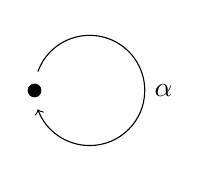
\begin{tikzpicture}
    \draw[fill = black] (-0.7 ,0) circle (0.08);
    \draw ([shift=(160 : 0.7)]0, 0) arc (160 : 0: 0.7) node [anchor = west] {$\alpha$};
    \draw[->] (0.7, 0)  arc (0 : -160 :  0.7);
    %\draw[-{libertinustip[length=5pt]}, thick] (-0.7, 0) arc (160 :  20   : 0.7);
    %\draw[thick] ( 0.7, 0) arc (0   : -180 : 0.7);
  \end{tikzpicture}
  \caption{The Jordan quiver~$Q$.}
  \label{jordan quiver}
\end{figure}
In the following we write~$\kf$ to mean a field or~$\Finite_1$.

A representation of the Jordan~quiver over~$\kf$ is the same as a pair~$(V,f)$ consisting of a~\vectorspace{$\kf$}~$V$ together with an endomorphism~$f$ of~$V$.
Two such representations~$(V, f)$ and~$(W, g)$ are isomorphic if and only if~$V$,~$W$ are isomorphic as~\vectorspaces{$\kf$} and the endomorphisms~$f$,~$g$ are similar.
We hence find that that the isomorphism classes of~\representations{$Q$} over~$\kf$ are in one-to-one correspondence to conjugacy classes of endomorphisms of~\vectorspaces{$\kf$}.

Suppose that~$V$ is finite-dimensional, and that~$\kf$ is algebraically closed, or that it is~$\Finite_1$, or that we are interested only in nilpotent endomorphisms.
Then one can use the usual Jordan normal form to classify these conjugacy classes.

A representation~$(V, f)$ of the Jordan quiver is nilpotent if and only if the endomorphism~$f$ is nilpotent.
We will in the rest of this talk restrict our attention to finite-dimensional, nilpotent representations of the Jordan quiver.
As introduced in the previous talks we denote by
\[
  \repnil(Q, \kf)
\]
the full subcategory of~$\Rep(Q, \kf)$ whose objects are the finite-dimensional, nilpotent representations of~$Q$ over~$\kf$.
We denote the set of isomorphism classes of~$\repnil(Q, \kf)$ by
\[
  \Iso(Q, \kf)
  \defined
  \repnil(Q, \kf) / {\cong} \,.
\]

\begin{definition}
  For every dimension~$d \geq 0$ let
  \[
    \Nil_d
    \defined
    \left(
      \kf^d,
      \begin{bmatrix}
        0 & 1       &         &   \\
          & \ddots  & \ddots  &   \\
          &         & \ddots  & 1 \\
          &         &         & 0
      \end{bmatrix}
    \right)
  \]
  if~$\kf$ is a field, and let
  \[
    \Nil_d
    \defined
    (
      \{ 0, 1, \dotsc, d \},
      [d \mapsto (d-1) \mapsto (d-2) \mapsto \dotsb \mapsto 1 \mapsto 0 \mapsto 0]
    )
  \]
  if~$\kf = \Finite_1$.
  For every tupel~$(d_1, \dotsc d_n)$ of dimensions~$d_i \geq 0$ let
  \[
    \Nil_{(d_1, \dotsc, d_n)}
    \defined
    \Nil_{d_1} \oplus \dotsb \oplus \Nil_{d_n} \,.
  \]
\end{definition}

\begin{example}  
  See \cref{nilpotent representation example} for visualizations of~$\Nil_{(4,3,3,2)}$ and~$\Nil_{(2,3,2,4,3)}$ over~$\Finite_1$.
  \begin{figure}[tb]
    \centering
      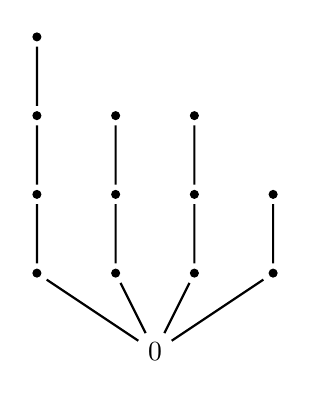
\begin{tikzpicture}
        % origin
        \node at (0,0) (Z) {$0$};
        % first line
        \node at (-1.5,1) (A1) {};
        \node at (-1.5,2) (A2) {};
        \node at (-1.5,3) (A3) {};
        \node at (-1.5,4) (A4) {};
        \draw[fill = black] (A1) circle (0.05);
        \draw[fill = black] (A2) circle (0.05);
        \draw[fill = black] (A3) circle (0.05);
        \draw[fill = black] (A4) circle (0.05);
        \draw[thick] (A4) -- (A3) -- (A2) -- (A1) -- (Z);
        % second line
        \node at (-0.5,1) (B1) {};
        \node at (-0.5,2) (B2) {};
        \node at (-0.5,3) (B3) {};
        \draw[fill = black] (B1) circle (0.05);
        \draw[fill = black] (B2) circle (0.05);
        \draw[fill = black] (B3) circle (0.05);
        \draw[thick] (B3) -- (B2) -- (B1) -- (Z);
        % third line
        \node at (0.5,1) (C1) {};
        \node at (0.5,2) (C2) {};
        \node at (0.5,3) (C3) {};
        \draw[fill = black] (C1) circle (0.05);
        \draw[fill = black] (C2) circle (0.05);
        \draw[fill = black] (C3) circle (0.05);
        \draw[thick] (C3) -- (C2) -- (C1) -- (Z);
        % fourth line
        \node at (1.5,1) (D1) {};
        \node at (1.5,2) (D2) {};
        \draw[fill = black] (D1) circle (0.05);
        \draw[fill = black] (D2) circle (0.05);
        \draw[thick] (D2) -- (D1) -- (Z);
      \end{tikzpicture}
      \qquad\qquad
      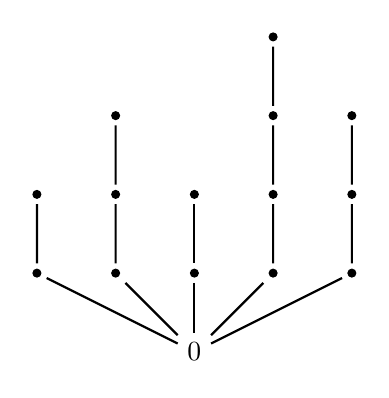
\begin{tikzpicture}
        % origin
        \node at (0,0) (Z) {$0$};
        % first line
        \node at (-2,1) (A1) {};
        \node at (-2,2) (A2) {};
        \draw[fill = black] (A1) circle (0.05);
        \draw[fill = black] (A2) circle (0.05);
        \draw[thick] (A2) -- (A1) -- (Z);
        % second line
        \node at (-1,1) (B1) {};
        \node at (-1,2) (B2) {};
        \node at (-1,3) (B3) {};
        \draw[fill = black] (B1) circle (0.05);
        \draw[fill = black] (B2) circle (0.05);
        \draw[fill = black] (B3) circle (0.05);
        \draw[thick] (B3) -- (B2) -- (B1) -- (Z);
        % third line
        \node at (-0,1) (C1) {};
        \node at (-0,2) (C2) {};
        \draw[fill = black] (C1) circle (0.05);
        \draw[fill = black] (C2) circle (0.05);
        \draw[thick] (C2) -- (C1) -- (Z);
        % fourth line
        \node at (1,1) (D1) {};
        \node at (1,2) (D2) {};
        \node at (1,3) (D3) {};
        \node at (1,4) (D4) {};
        \draw[fill = black] (D1) circle (0.05);
        \draw[fill = black] (D2) circle (0.05);
        \draw[fill = black] (D3) circle (0.05);
        \draw[fill = black] (D4) circle (0.05);
        \draw[thick] (D4) -- (D3) -- (D2) -- (D1) -- (Z);
        % fifth line
        \node at (2,1) (E1) {};
        \node at (2,2) (E2) {};
        \node at (2,3) (E3) {};
        \draw[fill = black] (E1) circle (0.05);
        \draw[fill = black] (E2) circle (0.05);
        \draw[fill = black] (E3) circle (0.05);
        \draw[thick] (E3) -- (E2) -- (E1) -- (Z);
      \end{tikzpicture}
      \caption{The representations~$\Nil_{(4,3,3,2)}$ and~$\Nil_{(2, 3, 2, 4, 3)}$ over~$\Finite_1$.}
    \label{nilpotent representation example}
  \end{figure}
\end{example}

\begin{definition}
  For every~$n \geq 0$ let~$\Par(n)$ be the set of partition of the number~$n$, i.e.\
  \[
    \Par(n)
    \defined
    \left\{
      (\lambda_1, \dotsc, \lambda_l)
    \suchthat*
      \begin{array}{@{}l@{}}
        \lambda_1, \dotsc, \lambda_l \in \Natural
        \\
        \lambda_1 \geq \dotsb \geq \lambda_l \geq 1
        \\
        \lambda_1 + \dotsb + \lambda_l = n
      \end{array}
      \spacing
    \right\} \,.%
    \footnote{
      We want to point out that in this talk we do not allow a partition to contain zero as an entry.
      This is done purely for technical reasons.
    }
  \]
  The set of all partitions is denoted by
  \[
    \Par
    \defined
    \coprod_{n \geq 0} \Par(n) \,.
  \]
\end{definition}

\begin{proposition}
  \label{representatives via partitions}
  The representations~$\Nil_\lambda$ with~$\lambda \in \Par$ form a set of representatives for~$\Iso(Q, \kf)$.
\end{proposition}

\begin{proof}
  This follows from the existence and uniqueness of the Jordan normal form of nilpotent endomorphisms.
  (See \cref{jordan normal form} for the Jordan normal form over~$\Finite_1$.)
\end{proof}





\section{The Hall~Algebra of the Jordan Quiver over~$\Finite_q$}

We will now consider for~$\kf$ the finite field~$\Finite_q$.
Then~$\repnil(Q, \Finite_q)$ is an abelian, finitary, full, exact subcategory of~$\Rep(Q, \Finite_q)$.
We want to consider in the following the Hall algebra of~$\repnil(Q, \Finite_q)$.
For this we need to understand its Euler form.

\begin{proposition}
  Let~$\Acat \defined \repnil(Q, \Finite_q)$ and let~$S \defined \Nil_1 = (\kf, [0])$.
  \begin{enumerate}
    \item
      The category~$\Acat$ is hereditary, i.e.~$\Ext^n_{\Acat} = 0$ for every~$n \geq 2$.
    \item
      The Grothendieck group~$\GrGr(\Acat)$ is freely generated by the class~$\class{S}$.
      Thus~$\GrGr(\Acat) \cong \Integer$ via the map~$\class{M} \mapsto \dim(M)$.
    \item
      The Euler form of~$\Acat$ vanishes.
  \end{enumerate}
\end{proposition}

\begin{proof}
  See \cref{proof of repnil is hereditary} and~\cref{proof of controlling ext}.
\end{proof}

Since~$\repnil(Q, \Finite_q)$ is abelian and finitary with vanishing Euler form we can consider its Hall algebra~$\Hall(Q, \Finite_q)$.
We find that Green’s coproduct makes~$\Hall(Q, \Finite_q)$ into a graded bialgebra because~$\repnil(Q, \Finite_q)$ satisfies the finite subject condition and has vanishing Euler form.%
\footnote{%
  We say that a category~$\Acat$ satisfies the \defemph{finite subobject condition} if every object of~$\Acat$ admits only finitely many subobjects.
}
It further follows that~$\Hall(Q, \Finite_q)$ is a graded Hopf algebra since it is connected.
(See \cref{explicit description of hall algebra over Fq} for a more detailed overview.)

The Hall algebra~$\Hall(Q, \Finite_q)$ has the classes~$\class{\Nil_\lambda}$ with~$\lambda \in \Par$ as a basis.
The multiplication of~$\Hall(Q, \Finite_q)$ is given by
\[
  \class{\Nil_\lambda} \cdot \class{\Nil_\mu}
  =
  \sum_{\nu \in \Par}
  F^\nu_{\lambda, \mu} \class{\Nil_\nu}
\]
where the structure constants~$F^\nu_{\lambda, \mu}$ are given by
\[
  F^\nu_{\lambda, \mu}
  =
  \counting
  \{
    \text{subrepresentation~$L$ of~$\Nil_\nu$}
  \suchthat
    L \cong \Nil_\mu,
    \Nil_\nu/L \cong \Nil_\lambda
  \} \,.
\]
We will now compute some of the structure constants, following \cite[Example~2.2]{schiffmann_hall}.

\begin{example}[Structure constants]
  \leavevmode
  \begin{enumerate}
    \item
      Let~$\lambda = (1^n)$ and~$\mu = (1^m)$.
      We consider the partition~$\nu \defined (1^{n+m})$.
      The action of the edge of the Jordan quiver~$Q$ on the representations~$\Nil_\lambda$,~$\Nil_\mu$ and~$\Nil_\nu$ is trivial.
      We thus find that every~\dimensional{$m$} linear subspace~$L$ of~$\Nil_{\nu}$ satisfies the conditions~$L \cong \Nil_\mu$ and~$\Nil_\nu / L \cong \Nil_\lambda$.
      The structure constant~$F^{\nu}_{\lambda, \mu}$ is therefore given by
      \begin{align*}
        F^{\nu}_{\lambda, \mu}
        &=
        \text{number of~\dimensional{$m$} linear subspaces of~$\Nil_{\nu}$}
        \\
%        &=
%        \text{number of~\dimensional{$m$} linear subspaces of~$\Finite_q^{n+m}$}
%        \\
        &=
        \counting {\Gr(m, n+m, \Finite_q)}
        \\
        &=
        \qbinom{n+m}{m}_q \,.
      \end{align*}
      (See \cref{size of quantum grassmannian} for the last equality.)
      We see in particular that~$F^{\nu}_{\lambda, \mu}$ depends is a polynomial way on~$q$ (with natural coefficients). 
      See \cref{examples of quantum binomial coefficients} for some explicit calculations of binomial coefficients.
    \item
      Let now~$\lambda = (n)$ and~$\mu = (m)$.
      We consider the partition~$\nu = (n+m)$. 
      The representation$~\Nil_{\nu}$ has the standard basis~$e_1, \dotsc, e_{n+m}$, and the subrepresentations of~$\Nil_{\nu}$ are given by~$\gen{e_1, \dotsc, e_i}$ for~$i = 0, \dotsc, n+m$.
      The subrepresentations~$L \defined \gen{e_1, \dotsc, e_m}$ is the unique one that is isomorphic to~$\Nil_\mu$, and its quotient~$\Nil_\nu / L$ is isomorphic to~$\Nil_\lambda$.
      Thus
      \[
        F^{(n+m)}_{(n),(m)}
        =
        1 \,.
      \]
    \item
      One finds for all~$n \geq 2$ and~$m \geq 1$ that
      \[
        F^{(n, 1^m)}_{(n), (1^m)}
        =
        q^m
        =
        F^{(n, 1^m)}_{(1^m), (n)} \,,
      \]
      see \cref{computing more structure constants}.
  \end{enumerate}
  We observe that in the above examples the coefficient~$F^{\nu}_{\lambda, \mu}$ are always polynomials in~$q$ with integer coefficients.
  We will see in next week’s talk that this is true for any coefficient~$F^{\nu}_{\lambda, \mu}$.
  This will allow us to define the \defemph{generic Hall algebra} of the Jordan quiver.

  We also have~$F^{\nu}_{\lambda, \mu} = F^{\nu}_{\mu, \lambda}$ in each example.
  We will see in next week’s talk that the Hall algebra~$\Hall(Q, \Finite_q)$ is indeed commutative, which means precisely that~$F^\nu_{\lambda, \mu} = F^\nu_{\mu, \lambda}$ for any three partitions~$\lambda, \mu, \nu \in \Par$.
\end{example}





\section{The Hall~Algebra of the Jordan Quiver over~$\Finite_1$}

We will now consider the case that~$\kf$ is~$\Finite_1$.
We have seen in last week’s talk how to construct the Hall algebra of~$Q$ over~$\Finite_1$, and that it is a cocommutative, graded Hopf algebra.
(See \cref{explicit description of hall algebra over F1} for a more detailed overview.)

We have also seen that~$\Hall(Q, \Finite_1)$ is the universal enveloping algebra of its Lie algebra of its primitve elements, which is spanned (as a vector space) by those isomorphism classes~$\class{M}$ for which~$M$ is indecomposable.
We have the following consequence:

\begin{corollary}
  \label{hall algebra generators}
  The Hall algebra~$\Hall(Q, \Finite_1)$ is generated by~$\class{\Nil_i}$ for~$i \geq 1$.
\end{corollary}

A more explicit proof of \cref{hall algebra generators} can be found in \cref{indecomposables generate hall algebra}.

\begin{example}[Structure constants]
  \label{computing multiplication over F1}
  We can again compute some structure constants~$F^\nu_{\lambda, \mu}$.
  \begin{enumerate}
    \item
      Let again~$\lambda = (1^n)$ and~$\mu = (1^m)$, and consider~$\nu = (1^{n+m})$.
      We find as before that
      \[
        F^{\nu}_{\lambda, \mu}
        =
        \text{number of~\dimensional{$m$} subspaces of~$\Nil_{n+m}$}
        =
        \binom{n+m}{m} \,.
      \]
%      This is the same result as before by taking the limit~$q \to 1$.
    \item
      Let again~$\lambda = (n)$ and~$\mu = (m)$ and consider~$\nu = (n+m)$.
      We find as before that
      \[
        F^{\nu}_{\lambda, \mu} = 1 \,.
      \]
    \item
      Let us compute the product~$\class{\Nil_i} \cdot \class{\Nil_j}$.

      We observe that if~$\class{R} \in \Iso(Q, \Finite_1)$ and~$L$ is a subrepresentation of~$R$ that is isomorphic to~$\Nil_j$ then the quotient~$R/L$ results from~$R$ by contracting one of the Jordan chains of~$R$ by~$j$ elements.
      % TODO: Better formulation:
      If~$R/L \cong \Nil_i$ then this means that~$R$ consists of a single Jordan chain of length~$i+j$, or of two Jordan chains of length~$i$ and~$j$ respectively.
      Thus
      \[
        \class{\Nil_i} \cdot \class{\Nil_j}
        =
        a \class{ \Nil_{(i,j)} }
        +
        b \class{ \Nil_{i+j} } \,.
      \]
      We have seen above that~$b = F^{(i+j)}_{(i),(j)} = 1$.
      The coeffient~$a = F^{(i,j)}_{(i),(j)}$ is given by
      \begin{align*}
        a
        &=
        \text{how often~$j$ occurs in~$(i,j)$}
        \\
        &=
        \begin{cases*}
          1
          &
          if~$i \neq j$,
          \\
          2
          &
          if~$i = j$.
        \end{cases*}
      \end{align*}
      Thus
      \begin{equation}
        \label{computing product of two generators for representations}
        \class{\Nil_i} \cdot \class{\Nil_j}
        =
        \begin{cases*}
          \class{\Nil_{(i,j)}} + \class{\Nil_{i+j}}
          &
          if~$i \neq j$,
          \\
          2 \class{\Nil_{(i,j)}} + \class{\Nil_{i+j}}
          &
          if~$i = j$.
        \end{cases*}
      \end{equation}
      We see in particular that~$\class{\Nil_i}$ and~$\class{\Nil_j}$ commute.
  \end{enumerate}
\end{example}

\begin{corollary}
  The Hall algebra~$\Hall(Q, \Finite_1)$ is commutative.
\end{corollary}

\begin{proof}
  Its generators~$\class{\Nil_i}$ with~$i \geq 1$ commute.
\end{proof}

We see now that~$\Hall(Q, \Finite_1)$ is a commutative, cocommutative, graded Hopf algebra.
It has a basis indexed by partitions, and its graded parts have the dimension
\[
  \dim \Hall(Q, \Finite_1)_k
  =
  \counting
  \{
    (\lambda_1, \dotsc, \lambda_l) \in \Par
  \suchthat
    \lambda_1 + 2 \lambda_2 + \dotsb + l \lambda_l = k
  \}
\]
for every~$k \geq 0$.

In the land of combinatorics there is another algebra with these properties, namely the \emph{ring of symmetric functions}.





\section{The Ring of Symmetric Functions}



\subsection{Definition}

For every~$n \geq 0$ we denote by
\[
  \Lambda^{(n)}
  \defined
  \Complex[x_1, \dotsc, x_n]^{\symm_n}
\]
the algebra of symmetric polynomials in~$n$ variables.
We have for every number of variables~$n \geq 0$ a homomorphism of graded algebras
\[
  \Lambda^{(n+1)} \to \Lambda^{(n)} \,,
  \quad
  f^{(n+1)}
  \mapsto
  f^{(n+1)}(x_1, \dotsc, x_n, 0) \,.
\]

\begin{definition}
  The \defemph{ring of symmetric functions}~$\Lambda$ is the limit
  \[
    \Lambda
    \defined
    \lim_{n \geq 0}
    \Bigl( \Lambda^{(n+1)} \to \Lambda^{(n)} \Bigr)
  \]
  in the category of graded algebras.
  The elements of~$\Lambda$ are \defemph{symmetric functions}.
\end{definition}

\begin{warning}
  A symmetric function is -- contrary to its name -- not a function.
\end{warning}

Let us make the above definition more explicit:
For every degree~$k \geq 0$ we have
\begin{align*}
  \Lambda_k
  &=
  \lim_{n \geq 0}
  \Bigl( \Lambda^{(n+1)}_k \to \Lambda^{(n)}_k \Bigr)
  \\
  &=
  \left\{
    \bigl( f^{(n)} \bigr)_{n \geq 0}
    \suchthat*
    \begin{tabular}{@{}l@{}}
      $f^{(n)} \in \Lambda^{(n)}_k$ for every~$n \geq 0$ such that \\
      $f^{(n+1)}(x_1, \dotsc, x_n, 0) = f^{(n)}$ for every~$n \geq 0$
    \end{tabular}
  \right\} \,,
\end{align*}
and we have overall
\[
  \Lambda
  =
  \bigoplus_{k \geq 0} \Lambda_k
\]
as vector spaces.
A homogeneous symmetric function~$f$, say of degree~$k$, is thus the same as a \enquote{consistent choice} of homogeneous symmetric polynomials~$f^{(n)}$ of degree~$k$ for every number of variables~$n \geq 0$.
%The multiplication on~$\Lambda$ is given by
%\[
%  (f^{(n)})_{n \geq 0}
%  \cdot
%  (g^{(n)})_{n \geq 0}
%  =
%  (f^{(n)} \cdot g^{(n)})_{n \geq 0}
%\]
%for all homogeneous symmetric functions~$(f^{(n)})_{n \geq 0} \in \Lambda_k$ and~$(g^{(n)})_{n \geq 0} \in \Lambda_l$.

We have for every number of variables~$n \geq 0$ a homomorphism of graded algebras
\[
  \Lambda
  \to
  \Lambda^{(n)} \,,
  \quad
  f
  \mapsto
  f(x_1, \dotsc, x_n)
\]
that is given in each degree by projection onto the~\howmanyth{$n$} component.%
\footnote{%
  For any two symmetric functions~$f, g \in \Lambda$ we have by construction of the algebra~$\Lambda$ that~$f = g$ if and only if~$f(x_1, \dotsc, x_n) = g(x_1, \dotsc, x_n)$ for every number of variables~$n \geq 0$.
  It also sufficies that this equality holds for all sufficiently large~$n$, i.e.\ if there exists some~$N$ such that this equality holds for all~$n \geq N$.
}

\begin{example}
  We have for every number of variables~$n \geq 0$ and every degree~$k \geq 0$ the \defemph{elementary symmetric polynomial}
  \[
    e^{(n)}_k(x_1, \dotsc, x_n)
    \defined
    \sum_{1 \leq i_1 < \dotsb < i_k \leq n}
    x_{i_1} \dotsm x_{i_k}
    \in
    \Lambda^{(n)}_k \,,
  \]
  with~$e^{(n)}_k = 0$ whenever~$k > n$.
  These polynomials satisfy the compatibility condition
  \[
    e^{(n+1)}_k(x_1, \dotsc, x_n, 0)
    =
    e^{(n)}_k
  \]
  for all~$n \geq 0$.
  These elementary symmetric polynomials~$e^{(n)}_k$ with~$n \geq 0$ therefore assemble into a single homogeneous symmetric function
  \[
    e_k \in \Lambda_k \,.
  \]
  This is the~\defemph{\howmanyth{$k$} elementary symmetric function}. 

  We find similarly that the \defemph{power symmetric polynomials}
  \[
    p^{(n)}_k(x_1, \dotsc, x_n)
    \defined
    x_1^k + \dotsb + x_n^k \,,
  \]
  and the \defemph{complete homogenous symmetric polynomials}
  \[
    h^{(n)}_k(x_1, \dotsc, x_n)
    \defined
    \sum_{1 \leq i_1 \leq \dotsb \leq i_k \leq n}
    x_{i_1} \dotsm x_{i_k}
    =
    \sum \text{monomials of homogeneous degree~$k$}
  \]
  result in homogeneous symmetric functions
  \[
    p_k, h_k
    \in
    \Lambda_k \,.
  \]
  These are the \defemph{power symmetric functions} and \defemph{complete homogeneous symmetric functions}.
\end{example}

See \cref{wrong symmetric functions} for some remarks about the definition of~$\Lambda$.



\subsection{The Fundamental Theorem on Symmetric Functions}

The \defemph{fundamental theorem of symmetric polynomials} asserts that for every number of variables~$n \geq 0$ the elementary symmetric polynomials
\[
  e^{(n)}_1, \dotsc, e^{(n)}_n
\]
form an algebraically independent generating set for the algebra of symmetric polynomials~$\Lambda^{(n)}$.
It follows from this that both
\[
  h^{(n)}_1, \dotsc, h^{(n)}_n
  \quad\text{and}\quad
  p^{(n)}_1, \dotsc, p^{(n)}_n
\]
also form algebraically independent algebra generating set for~$\Lambda^{(n)}$.%
\footnote{
  For the elementary symmetric polynomials~$e^{(n)}_k$ and homogeneous symmetric polynomials~$h^{(n)}_k$ these statements do not only hold over the ground field~$\Complex$, but over every commutative ring.
  For the power symmetric polynomials~$p^{(n)}_k$ we need to work over a field in which the numbers~$1, \dotsc, n$ are invertible.
}

For every partition~$\lambda \in \Par$ with~$\lambda = (\lambda_1, \dotsc, \lambda_l)$ we can consider the symmetric polynomials
\[
  e^{(n)}_\lambda
  \defined
  e^{(n)}_{\lambda_1} \dotsm e^{(n)}_{\lambda_l} \,,
  \qquad
  h^{(n)}_\lambda
  \defined
  h^{(n)}_{\lambda_1} \dotsm h^{(n)}_{\lambda_l} \,,
  \qquad
  p^{(n)}_\lambda
  \defined
  p^{(n)}_{\lambda_1} \dotsm p^{(n)}_{\lambda_l} \,.
\]
We have just formulated that the symmetric polynomials
\[
  e^{(n)}_\lambda
  \qquad
  \text{for $\lambda \in \Par$ with length~$\length(\lambda) \leq n$}
\]
form a vector space basis for~$\Lambda^{(n)}$, and similarly for~$h^{(n)}_\lambda$ and~$p^{(n)}_\lambda$.
We can generalize these families of symmetric polynomials to symmetric functions:

\begin{example}
  For every partition~$\lambda \in \Par$ with~$\lambda = (\lambda_1, \dotsc, \lambda_l)$ we consider the symmetric functions
  \[
    e_\lambda
    \defined
    e_{\lambda_1} \dotsm e_{\lambda_l} \,,
    \quad
    h_\lambda
    \defined
    h_{\lambda_1} \dotsm h_{\lambda_l} \,,
    \quad
    p_\lambda
    \defined
    p_{\lambda_1} \dotsm p_{\lambda_l}
  \]
  and note that
  \begin{align*}
    \SwapAboveDisplaySkip
    e_\lambda(x_1, \dotsc, x_n)
    &=
    e^{(n)}_\lambda \,,
    \\
    h_\lambda(x_1, \dotsc, x_n)
    &=
    h^{(n)}_\lambda \,,
    \\
    p_\lambda(x_1, \dotsc, x_n)
    &=
    p^{(n)}_\lambda \,.
  \end{align*}
\end{example}

We now want to generalize the fundamental theorem on symmetric polynomials to symmetric functions.
The key observation behind this is the following:

\begin{proposition}
  \label{sequence stabilizes}
  The map~$\Lambda^{(n+1)}_k \to \Lambda^{(n)}_k$ is an isomorphism whenever~$n \geq k$. 
\end{proposition}

\begin{proof}
  A vector space basis of~$\Lambda^{(n)}_k$ is given by the symmetric polynomials~$e^{(n)}_\lambda$ where the partition~$\lambda$ is of length~$\length(\lambda) \leq n$ and~$\lambda = (\lambda_1, \dotsc, \lambda_l)$ satisfies
  \[
    \lambda_1 + 2 \lambda_2 + \dotsb + l \lambda_l = k \,.
  \]
  A vector space basis of~$\Lambda^{(n)}_k$ is given by the symmetric polynomials~$e^{(n+1)}_\mu$ where the partition~$\mu$ is of length~$\length(\mu) \leq n+1$ and~$\mu = (\mu_1, \dotsc, \mu_l)$ satisfies
  \[
    \mu_1 + 2 \mu_2 + \dotsb + l \mu_l = k \,.
  \]
  We find by degree reasons that the case~$\length(\mu) = n+1$ cannot occur.
  The linear map~$\Lambda^{(n+1)}_k \to \Lambda^{(n)}_k$ does therefore restrict to a bijection between the above bases.
\end{proof}

\begin{corollary}
  \label{iso in each degree for sufficiently large}
  The map~$\Lambda_k \to \Lambda^{(n)}_k$ is an isomorphism whenever~$n \geq k$.
  \qed
\end{corollary}

\begin{corollary}
  \label{bases for symmetric functions}
  The following families of symmetric functions form vector space bases of~$\Lambda$:
  \begin{enumerate}
    \item
      The elementary symmetric polynomials~$e_\lambda$ with~$\lambda \in \Par$.
    \item
      The complete homogeneous symmetric polynomials~$h_\lambda$ with~$\lambda \in \Par$.
    \item
      The power symmetric polynomials~$p_\lambda$ with~$\lambda \in \Par$.
    \qed
  \end{enumerate}
\end{corollary}

\begin{corollary}
  The elementary symmetric functions~$e_k$ with~$k \geq 1$ form an algebraically independent algebra generating set for~$\Lambda$, and similarly the~$h_k$ and the~$p_k$.
  \qed
\end{corollary}

\begin{corollary}
  We have~$\Lambda \cong \Complex[X_1, X_2, X_3, \dotsc]$ as graded algebras, where each variable~$X_k$ is homogeneous of degree~$k$.
  \qed
\end{corollary}

See \cref{symmetric functions as colimit} for more consequences.



\subsection{Hopf Algebra Structure}

We can endow the algebra of symmetric functions~$\Lambda$ with the structure of a graded Hopf algebra.
We have for any two number of variables~$n, m \geq 0$ a homomorphism of graded algebras
\begin{align*}
  \Delta_{nm}
  \colon
  \Lambda^{(n+m)}
  &=
  \Complex[x_1, \dotsc, x_{n+m}]^{\symm_{n+m}}
  \\
  &\subseteq
  \Complex[x_1, \dotsc, x_{n+m}]^{\symm_n \times \symm_m}
  \\
  &\cong
  ( \Complex[x_1, \dotsc, x_n] \tensor \Complex[x_{n+1}, \dotsc, x_{n+m}] )^{\symm_n \times \symm_m}
  \\
  &\cong
  ( \Complex[x_1, \dotsc, x_n] \tensor \Complex[x_1, \dotsc, x_m] )^{\symm_n \times \symm_m}
  \\
  &=
  \Complex[x_1, \dotsc, x_n]^{\symm_n} \tensor \Complex[x_1, \dotsc, x_m]^{\symm_m}
  \tag{\cref{invariants of tensor product}}
  \\
  &=
  \Lambda^{(n)} \tensor \Lambda^{(m)}.
\end{align*}
We would like to have a homomorphism of graded algebras~$\Delta \colon \Lambda \to \Lambda \tensor \Lambda$ such that for any number of variables~$n, m \geq 0$ the square diagram
\[
  \begin{tikzcd}
    \Lambda
    \arrow[dashed]{r}[above]{\Delta}
    \arrow{d}
    &
    \Lambda \tensor \Lambda
    \arrow{d}
    \\
    \Lambda^{(n+m)}
    \arrow{r}[above]{\Delta_{nm}}
    &
    \Lambda^{(n)} \tensor \Lambda^{(m)}
  \end{tikzcd}
\]
commutes.
The composition~$\Lambda \to \Lambda^{(n)} \tensor \Lambda^{(m)}$ is given on the algebra generators~$p_k$ of~$\Lambda$ by
\[
  p_k \mapsto p^{(n)}_k \tensor 1 + 1 \tensor p^{(m)}_k \,.
\]
Such an algebra homomorphism~$\Delta$ is thus given by
\[
  \Delta(p_k) = p_k \tensor 1 + 1 \tensor p_k \,.  
\]
This homomorphism exists because~$\Lambda$ is the free commutative algebra on the generators~$p_k$.
% TODO: Uniqueness?

The homomorphism~$\Delta$ makes the algebra~$\Lambda$ into a cocommutative, graded bialgebra.
%The counit is given on algebra generators by
%\[
%  \varepsilon(p_k) = 0
%\]
%for every~$k \geq 0$.
Since~$\Lambda$ is graded and connected it follows that it is already a graded Hopf algebra.
%Its antipode is given on algebra generators by
%\[
%  S(p_k) = -p_k
%\]
%for every~$k \geq 0$.

We see altogether that~$\Lambda$ is a commutative, cocommutative, graded Hopf algebra.
It has a basis indexed by partitions, and its graded parts have the dimension
\[
  \dim \Lambda_k
  =
  \counting
  \{
    (\lambda_1, \dotsc, \lambda_l) \in \Par
  \suchthat
    \lambda_1 + 2 \lambda_2 + \dotsb + l \lambda_l
    =
    k
  \} \,.
\]





\section{The Isomorphism~$\Hall(Q, \Finite_1) \cong \Lambda$}
\label{the isomorphism}

Both~$\Hall(Q, \Finite_1)$ and~$\Lambda$ are commutative, cocommutate, graded Hopf algebras.
They are isomorphic as graded Hopf Algebras:

The ring of symmetric functions~$\Lambda$ is, as a commutative algebra, freely generated by the power symmetric functions~$p_1, p_2, p_3, \dotsc$
There hence exists a unique, surjective algebra homomorphism~$\Phi \colon \Lambda \to \Hall(Q, \Finite_1)$ with
\[
  \Phi(p_k) = \class{\Nil_k}
\]
for every degree~$k \geq 1$.
We note that~$\Phi$ is a homomorphism of graded algebras because both~$p_i$ and~$\class{ \Nil_k }$ are of degree~$k$.
We also have for every degree~$k \geq 0$ that~$\dim \Lambda_k = \dim \Hall(Q, \Finite_1)_k$, with this dimension being finite.
It thus follows from the surjectivity of~$\Phi$ that it is already an isomorphism of graded algebras.

The algebra isomorphism~$\Phi$ is already an isomorphism of Hopf algebras:
It sufficies to check that~$\Phi$ is compatible with the comultiplication of the algebra generators~$p_k$.
This holds since~$p_k$ is primitive in~$\Lambda$ and~$\class{ \Nil_k }$ is primitive in~$\Hall(Q, \Finite_1)$.

We have shown altogether that~$\Phi$ is an isomorphism of graded Hopf algebras.

\begin{remark}
  For every partition~$\lambda = (\lambda_1, \dotsc, \lambda_l)$ one can generalize the monomial symmetric polynomials
  \[
    m^{(n)}_\lambda(x_1, \dotsc, x_n)
    =
    \sum \text{distinct permutations of~$x_1^{\lambda_1} \dotsm x_l^{\lambda_l}$}
  \]
  to symmetric functions~$m_\lambda$.
  See \cref{monomial symmetric functions} for more details.

  One has~$m_{(k)} = p_k$ for every~$k \geq 1$, and therefore
  \[
    \Phi( m_{(k)} )
    =
    \Phi(p_k)
    =
    \class{ \Nil_k } \,.
  \]
  One can check (by hand) that
  \[
    m_{(i)} \cdot m_{(j)}
    =
    \begin{cases*}
      m_{(i,j)} + m_{(i+j)}
      &
      if~$i \neq j$,
      \\
      2 m_{(i,j)} + m_{(i+j)}
      &
      if~$i = j$.
    \end{cases*}
  \]
  It then follows together with~\eqref{computing product of two generators for representations} from \cref{computing multiplication over F1} that
  \[
    \Phi( m_{(i,j)} )
    =
    \class{ \Nil_{(i,j)} }
  \]
  for any partition~$(i,j)$.
  It can be shown more generally that
  \[
    \Phi( m_\lambda )
    =
    \class{ \Nil_\lambda }
  \]
  for every partition~$\lambda \in \Par$, see \cref{understanding the iso on a basis}.
  Under the isomorphism~$\Phi$ the standard basis~$\class{\Nil_\lambda}$ of~$\Hall(Q, \Finite_1)$ does therefore correspond to the monomial symmetric functions~$m_\lambda$.
\end{remark}





\newpage
\appendix
\section{Remarks and Proofs}



\subsection{Theorem of Krull--Remak--Schmidt and Jordan Normal Form}
\label{jordan normal form}

Let~$V$ be an~\vectorspace{$\Finite_1$} and let~$f \colon V \to V$ be an endomorphism.

\begin{recall}
  \begin{enumerate}
    \item
      A \defemph{subspace} of~$V$ is a subset of~$V$ that contains the base point~$0$.
    \item
      If~$(U_i)_{i \in I}$ is a collection of subspaces of~$V$ then~$V = \bigoplus_{i \in I} U_i$ if and only if every nonzero evement of~$V$ is contained in precisely one~$U_i$, i.e.\ if and only if the~$U_i$ give a disjoint decomposition of the set~$V \setminus \{ 0 \}$.
    \item
      If~$U$ is a subspace of~$V$ and~$V = \bigoplus_{i \in I} W_i$ is a direct sum decomposition then~$U = \bigoplus_{i \in I} (U \cap W_i)$.
  \end{enumerate}
\end{recall}

\begin{definition}
  A subspace~$U$ of~$V$ is~\defemph{\invariant{$f$}} if~$f(U) \subseteq U$.
  An~\invariant{$f$} subspace~$U$ of~$V$ is \defemph{indecomposable} if it is nonzero and there exist no two nonzero~\invariant{$f$} subspaces~$W_1$,~$W_2$ of~$U$ with~$U = W_1 \oplus W_2$.
\end{definition}

\begin{remark}
  If~$U$ is an indecomposable subspace of~$V$ and~$U = \bigoplus_{i \in I} W_i$ is any decomposition into~\invariant{$f$} subspaces~$W_i$ then it follows that~$U = W_j$ for some~$j \in I$ while~$W_i = 0$ for every~$i \neq j$.
  Indeed, some~$W_j$ must be nonzero because~$V$ is nonzero.
  Then~$V = W_j \oplus \bigoplus_{i \in I, i \neq j} W_i$ and thus~$\bigoplus_{i \in I, i \neq j} W_i = 0$, and therefore~$W_i = 0$ for every~$i \in I$.
\end{remark}

\begin{proposition}[Krull--Remak--Schmidt]
  There exists a unique direct sum decomposition of~$V$ into indecomposable~\invariant{$f$} subspaces.
\end{proposition}

\begin{proof}
  In the following we mean by a \defemph{decomposition} a direct sum decomposition into~\invariant{$f$} subspaces in which each direct summand is nonzero.
  We say that a decomposition~$V = \bigoplus_{i \in I} U_i$ is \defemph{finer} than a decomposition~$V = \bigoplus_{j \in J} W_j$ if each~$U_i$ is contained in some~$W_j$.
  This gives a partial order on the set of decompositions of~$V$.

  We note that a decomposition~$V = \bigoplus_{i \in I} U_i$ consists of indecomposables if and only if it is maximal fine.
  Indeed, if some~$U_j$ is decomposable then there exists a decomposition~$U_j = U_j' \oplus U_j''$.
  Then
  \[
    V
    =
    \bigoplus_{i \in I} U_i
    =
    \bigoplus_{\substack{i \in I \\ i \neq j}} U_i \oplus U_j
    =
    \bigoplus_{\substack{i \in I \\ i \neq j}} U_i \oplus U_j' \oplus U_j'
  \]
  with the last term being a strictly finer that the original decomposition~$V = \bigoplus_{i \in I} U_i$.
  Suppose on the other hand that each~$U_i$ is indecomposable and that~$V = \bigoplus_{j \in J} W_j$ is a decomposition that is finer than~$V = \bigoplus_{i \in I} U_i$.
  Then~$U_i = \bigoplus_{j \in J} (U_i \cap V_j)$ for every~$j \in J$.
  It follows that~$U_i = U_i \cap V_j$ for some~$j \in J$ and thus~$U_i \subseteq V_j$.
  We also know that~$V_j$ is contained in some~$U_k$.
  Then~$U_i$ is contained in~$U_k$ whence it follows that~$i = k$ and thus~$U_i = V_j$.
  This shows that each~$U_i$ equals some~$V_j$, from which it follows that both decompositions must coincide.

  We hence need to show that there exists a unique decomposition which is maximal fine.
  It sufficies to show that any collection of decompositions has a common refinement.
  Taking a common refinement of all decompositions then gives the desired one.

  Let~$V = \bigoplus_{j \in J_i} U^i_j$ with~$i \in I$ be a collection of decompositions.
  For every nonzero vector~$v \in V$ there exists for every~$i \in I$ a unique index~$j(i,v) \in J_i$ with~$v \in U^i_{j(i,v)}$.
  We consider
  \[
    W_v
    \defined
    \bigcap_{i \in I} U^i_{j(i,v)} \,.
  \]
  Each~$W_v$ is an intersection of~\invariant{$f$} subspaces and therefore again an~\invariant{$f$} subspace.
  Each nonzero vector~$v$ of~$V$ is contained in some~$W_{v'}$, namely for~$v' = v$.

  Suppose that for two nonzero vectors~$v, u \in V$ the subspaces~$W_v$ and~$W_u$ intersect nonzero.
  Let~$w$ be a nonzero vector contained in both~$W_v$ and~$W_u$.
  Then for every index~$i \in I$ the vector~$w$ is contained in~$U^i_{j(i,v)}$, whence~$j(i,v) = j(i,w)$.
  It follows that~$W_v = W_w$, and we find in the same way that~$W_u = W_w$.
  Thus~$W_v = W_w$.

  This shows that the~\invariant{$f$} subspaces~$W_v$ give a disjoint decomposition of~$V \setminus \{0\}$, and hence a decomposition of~$V$.
  (Once we remove those subspaces which occur multiple times.)
  This decomposition of~$V$ is by construction finer than each decomposition~$V = \bigoplus_{j \in J_i} U^i_j$.
\end{proof}

We want to understand how the decomposition from the Krull--Remak--Schmidt theorem looks like.
We note that if~$v \in V$ is any nonzero vector then there exists at most one preimage of~$v$ under~$f$, since~$f$ is injective outside of its kernel.
Thus we can consider for every nonzero vector~$v \in V$ the well-defined two-sided sequence
\[
  \dotsc, f^{-2}(v), f^{-1}(v), v, f(v), f^2(v), \dotsc
\]
Here the left part of the sequence consists of as many iterated preimages as exist.
The set of all these elements is the \defemph{orbit} of~$v$ under~$f$.
It is denoted by~$\orbit{v}$.

We note that for any nonzero veector~$u$ in~$\orbit{v}$ we have~$\orbit{u} = \orbit{v}$.
If two orbits~$\orbit{v}$ and~$\orbit{w}$ intersect in a nonzero vector~$u$ then it follows that~$\orbit{v} = \orbit{u} = \orbit{v}$.
Two distinct orbit do therefore intersect at most in~$0$.
It follows that the orbits give induce a disjoint decomposition of~$V \setminus \{0\}$.
The vector space~$V$ does therefore decompose into the direct sum of the subspaces~$\orbit{v} \cup \{ 0 \}$.
(Once we remove those subspaces which occur multiple times.)
Each subspace~$\orbit{v} \cup \{ 0 \}$ is~\invariant{$f$}.
Any two nonzero~\invariant{$f$} subspaces of~$\orbit{v} \cup \{ 0 \}$ intersect nonzero whence the subspaces~$\orbit{v} \cup \{ 0 \}$ are indecomposable.

This shows that the decomposition of~$V$ from the Krull--Remak--Schmidt theorem is given by the orbits with respect to~$f$ (together with~$\{ 0 \}$).

There exist five kinds of orbits.
\begin{enumerate}[label = Type~\Alph*.]
  \item
    \label{finite nilpotent orbit}
    The orbit ends in zero and is finite:
    It is thus of the form
    \[
      v
      \to
      f(v)
      \to
      \dotsb
      \to
      f^n(v)
      =
      0
    \]
    for a unique vector~$v$, that has no preimage under~$f$.
  \item
    \label{infinite nilpotent orbit}
    The orbit ends in zero and is infintite:
    It is thus of the form
    \[
      \dotsb
      \to
      f^{-2}(v)
      \to
      f^{-1}(v)
      \to
      v
      \to
      f(v)
      \to
      f^2(v)
      \to
      \dotsb
      \to
      f^n(v)
      =
      0 \,.
    \]
  \item
    \label{infinite onesided}
    The orbit never reaches zero and has only finitely many preimages.
    It is thus of the form
    \[
      v
      \to
      f(v)
      \to
      f^2(v)
      \to
      \dotsb
      \to
      f^n(v)
      \to
      \dotsb
    \]
    for a unique vector~$v$, that has no preimage under~$f$.
  \item
    \label{infinite twosided orbit}
    The orbit goes infinite in both directions and is non-circular.
    It is thus of the form
    \[
      \dotsb
      \to
      f^{-1}(v)
      \to
      v
      \to
      f(v)
      \to
      f^2(v)
      \to
      \dotsb
      \to
      f^n(v)
      \to
      \dotsb
    \]
  \item
    \label{circle orbit}
    The orbit is circular.
    It is thus of the form
    \[
      v
      \to
      f(v)
      \to
      f^2(v)
      \to
      \dotsb
      \to
      f^n(v)
      \to
      v
      \to
      f(v)
      \to
      \dotsb
    \]
\end{enumerate}

Depending on the properties of the vector space~$V$ and endomorphism~$f$ not all kinds of orbits can occur.
\begin{itemize}
  \item
    The endomorphism~$f$ is injective if and only if no orbits of Type~A and Type~B occur.
  \item
  The endomorphism~$f$ is surjective if and only if no orbits of Type~A and Type~C occur.
  \item
    The endomorphism~$f$ is bijective if and only if only orbits of Type~D and Type~E occur.
  \item
    The endomorphism~$f$ is locally nilpotent if and only if only orbits of Type~A and Type~B appear.%
    \footnote{
      An endomorphism~$f$ is locally nilpotent if there exists for every vector~$v$ some power~$n \geq 0$ such that~$f^n(v) = 0$.
    }
  \item
    The endomorphism~$f$ is nilpotent if and only if only orbits of Type~A occur, and the lengths of the occuring orbits is bounded.
  \item
    If~$V$ is finite-dimensional then only orbits of Type~A and Type~E occur.
  \item
    More generally,~$V$ is locally finite-dimensional with respect to~$f$ if and only if only orbits of Type~A and Type~E occur.%
    \footnote{
      We say that~$V$ is locally finite-dimensional if every nonzero vector of~$V$ is contained in a finite-dimensional~\invariant{$f$} subspace.
    }
\end{itemize}
See \cref{orbit table} for an overview.
\begin{table}
  \centering
  \begin{tabular}{@{}lcccccc@{}}
      \toprule
    %
      {}
      &
      injective
      &
      surjective
      &
      bijective
      &
      nilpotent
      &
      finite-dimensional
    \\
      \midrule
    %
      Type~A
      &
      {}
      &
      {}
      &
      {}
      &
      \textopenbullet
      &
      \textopenbullet
    \\
      Type~B
      &
      {}
      &
      {}
      &
      \textbullet
      &
      \textopenbullet
      &
      {}
    \\
      Type~C
      &
      \textbullet
      &
      {}
      &
      {}
      &
      {}
      &
      {}
    \\
      Type~D
      &
      \textbullet
      &
      \textbullet
      &
      \textbullet
      &
      {}
      &
      {}
    \\
      Type~E
      &
      \textbullet
      &
      \textbullet
      &
      \textbullet
      &
      {}
      &
      \textopenbullet{}
%    \\
%      \midrule
%    %
%      \begin{tabular}{@{}c@{}}
%        additional\\
%        condition
%      \end{tabular}
%      &
%      {}
%      &
%      {}
%      &
%      {}
%      &
%      {}
%      &
%      \begin{tabular}{@{}c}
%        bounded \\
%        size of \\
%        orbits
%      \end{tabular}
%      &
%      \begin{tabular}{c@{}}
%        finite \\
%        number \\
%        of orbits
%      \end{tabular}
    \\
      \bottomrule
  \end{tabular}
  \caption{
    Possible orbits.
    Complete characterization via orbits for~\textbullet.
    Only locally for~\textopenbullet.
  }
  \label{orbit table}
\end{table}



%\subsection{Nilpotent Representations}
%\label{recalling nilpotent representations}
%
%A representation~$V = ((V_i)_{i \in \Gamma_0}, (f_\alpha)_{\alpha \in \Gamma_1})$ of a quiver~$\Gamma = (\Gamma_0, \Gamma_1)$ is \defemph{nilpotent} if there exists some~$N \geq 0$ such that for every path~$\alpha_n, \dotsc, \alpha_1$ in~$\Gamma$ of length~$n \geq N$ we have~$f_{\alpha_n} \circ \dotsb \circ f_{\alpha_1} = 0$.
%(See \cite[Definition~4.4]{quiver_reps_F1}.)
%
%If~$\Gamma$ is finite and has no oriented cycles then every representation of~$\Gamma$ is nilpotent.



\subsection{Proving that~$\repnil(Q, \Finite_q)$ is hereditary}
\label{proof of repnil is hereditary}

\begin{definition}
  Let~$\Acat$ be an abelian category.
  A subcategory~$\Bcat$ is \defemph{closed under extensions} if for every short exact sequence~$0 \to A \to B \to C \to 0$ in~$\Acat$ the middle term~$B$ is contained in~$\Bcat$ provided that both outer terms~$A$,~$C$ are contained in~$\Bcat$.
\end{definition}

\begin{definition}
  Let~$\Acat$ be an abelian category.
  A subcategory~$\Bcat$ of~$\Acat$ is a \defemph{Serre subcategory} if it is abelian, exact, full and closed under extensions.
\end{definition}

\begin{example}
  \label{repnil is a serre subcategory}
  The category~$\repnil(Q, \Finite_q)$ is a Serre subcategory of~$\Rep(Q, \Finite_q) \cong \Mod{\Finite_q[x]}$.
  Indeed, it is a full, abelian, exact subcategory of~$\Rep(Q, \Finite_q)$.
  If in a short exact sequence
  \[
    0
    \to
    A
    \xlongto{\varphi}
    B
    \xlongto{\psi}
    C
    \to
    0
  \]
  of~\representations{$Q$} both~$A$,~$B$ are finite-dimensional then the same holds for~$B$.
  If both~$A$,~$C$ are nilpotent then same holds for~$B$:
  There exists some powers~$n, m \geq 0$ with~$\alpha^n A = 0$ and~$\alpha^m C = 0$.
  It follows that~$\alpha^m B \subseteq \ker(\psi) = \im(\varphi)$ and thus~$\alpha^{n+m} B = 0$.
\end{example}

If~$\Acat$ is an abelian category and~$\Bcat$ is an abelian, exact subcategory then we have for every~$n \geq 0$ and every two objects~$A$,~$B$ of~$\Bcat$ an induced map
\[
  \Ext^n_{\Bcat}(A,B)
  \to
  \Ext^n_{\Acat}(A,B) \,.
\]

\begin{proposition}
  \label{ext for serre subcategories}
  Let~$\Acat$ be an abelian category and let~$\Bcat$ be an abelian, exact subcategory of~$\Acat$.
  \begin{enumerate}
    \item
      Suppose that~$\Bcat$ is a full subcategory of~$\Acat$.
      Then the induced map~$\Ext^1_{\Bcat}(A,B) \to \Ext^1_{\Acat}(A,B)$ is injective for any two objects~$A$,~$B$ of~$\Bcat$.
      If~$\Bcat$ is a Serre subcategory of~$\Acat$ then the induced map~$\Ext^1_{\Bcat}(A,B) \to \Ext^1_{\Acat}(A,B)$ is bijective.
    \item
      Suppose that~$\Bcat$ is a Serre subcategory of~$\Acat$.
      Suppose furthermore that for some~$n \geq 1$ the induced map~$\Ext^n_{\Bcat}(A,B) \to \Ext^n_{\Acat}(A,B)$ is bijective for any two objects~$A$,~$B$ of~$\Bcat$.
      Then the induced map~$\Ext^{n+1}_{\Bcat}(A,B) \to \Ext^{n+1}_{\Acat}(A,B)$ is injective for any two objects~$A$,~$B$ of~$\Bcat$. 
  \end{enumerate}
\end{proposition}


\begin{proof}
  \leavevmode
  \begin{enumerate}
    \item
      Two short exact sequences in~$\Bcat$,
      \[
        0 \to B \to X \to A \to 0
        \qquad\text{and}\qquad
        0 \to B \to X' \to A \to 0 \,,
      \]
      are equivalent in~$\Acat$ if there exists an isomorphism~$\varphi \colon X \to X'$ that makes the diagram
      \[
        \begin{tikzcd}
            0
            \arrow{r}
          &
            B
            \arrow{r}
            \arrow[equal]{d}
          &
            X
            \arrow{r}
            \arrow{d}[right]{\varphi}
          &
            A
            \arrow{r}
            \arrow[equal]{d}
          &
            0
          \\
            0
            \arrow{r}
          &
            B
            \arrow{r}
          &
            X'
            \arrow{r}
          &
            A
            \arrow{r}
          &
            0
        \end{tikzcd}
      \]
      commute.
      We find that~$\varphi$ is already an isomorphism in~$\Bcat$ because~$\Bcat$ is full in~$\Acat$.
      Thus both sequences are already equivalent in~$\Bcat$.
      This shows the injectivity of~$\Ext^1_{\Bcat}(A,B) \to \Ext^1_{\Acat}(A,B)$.

      Suppose now that~$\Bcat$ is a Serre subcategory of~$\Acat$.
      Let~$A$,~$B$ be two objects in~$\Bcat$.
      Every element~$\xi$ of~$\Ext^1_{\Acat}(A,B)$ is represented by a short exact sequence~$0 \to B \to X \to A \to 0$ in~$\Acat$.
      The middle term~$X$ is already contained in~$\Bcat$ because~$\Bcat$ is closed under extensions.
      Thus~$\xi$ lies in~$\Ext^1_{\Bcat}(A,B)$.
    \item
      We refer to \cite[Proposition~3.3]{yoneda_ext}.
    \qedhere
  \end{enumerate}
\end{proof}

\begin{corollary}
  \label{serre subcategories are again hereditary}
  Let~$\Acat$ be an abelian category and let~$\Bcat$ be a Serre subcategory of~$\Acat$.
  If~$\Acat$ is hereditary then so is~$\Bcat$.
\end{corollary}

\begin{proof}
  Let~$A$,~$B$ be two objects of~$\Bcat$.
  We show by induction on~$n \geq 1$ that the induced map~$\Ext^n_{\Bcat}(A,B) \to \Ext^n_{\Acat}(A,B)$ is bijective.
  The assertion follows from this.

  We know from \cref{ext for serre subcategories} that the induced map~$\Ext^1_{\Bcat}(A,B) \to \Ext^1_{\Acat}(A,B)$ is bijective.
  If for some~$n \geq 1$ the induced map~$\Ext^n_{\Bcat}(A,B) \to \Ext^n_{\Acat}(A,B)$ is bijective then it follows from \cref{ext for serre subcategories} that the induced map~$\Ext^{n+1}_{\Bcat}(A,B) \to \Ext^{n+1}_{\Acat}(A,B)$ is injective.
  It is also surjective because~$\Acat$ is hereditary.
\end{proof}

\begin{example}
  \Cref{repnil is a serre subcategory} shows that~$\repnil(Q, \Finite_q)$ is a Serre subcategory of~$\Rep(Q, \Finite_q)$.
  The category~$\Rep(Q, \Finite_q) \cong \Mod{\Finite_q[x]}$ is hereditary because it has enough projectives and submodules of projective~\modules{$\Finite_q[x]$} are again projective, since~$\Finite[x]$ is a principal ideal domain.
  It thus follows from \cref{serre subcategories are again hereditary} that~$\repnil(Q, \Finite_q)$ is again hereditary.
\end{example}



\subsection{Understanding~$\GrGr(\repnil(Q, \Finite_q))$ and the Euler Form of~$\repnil(Q, \Finite_q)$}
\label{proof of controlling ext}

The indecomposable objects of~$\repnil(Q, \Finite_q)$ are precisely~$\Nil_i$ with~$i \geq 1$.
The representation~$\Nil_i$ has (up to isomorphism) precisely the subrepresentations~$\Nil_j$ with~$j = 0, \dotsc, i$.
Thus~$\Nil_1$ is the unique simple object in~$\repnil(Q, \Finite_q)$.

Every objects in~$\repnil(Q, \Finite_q)$ admits a composition series, whose composition factors are necessarily the unique simple objects~$S$.
It follows that~$\class{S}$ is a free generator of the Grothendieck group~$K \defined \GrGr(\repnil(Q, \Finite_q))$.

We have~$\Hom(S, S) \cong \Finite_q$ and~$\Ext^1(S,S) \cong \Finite_q$.
The first isomorphism holds because~$S$ is one-dimensional, and the second is shown in \cref{computing ext}.

To show that the Euler form of~$\repnil(Q, \Finite_q)$ vanishes we regard it as a bilinear form
\[
  \euler{-}{-}
  \colon
  K \times K
  \to
  \Rational^\times \,.
\]
Since~$S$ is a generator of~$K$ is sufficies to show that~$\euler{S}{S} = 1$.
This holds true because
\[
  \euler{S}{S}
  =
  \Bigl( \counting {\Hom(S,S)} \Bigr)
  \cdot
  \Bigl( \counting \Ext^1(S,S) \Bigr)^{-1}
  =
  q \cdot q^{-1}
  =
  1 \,.
\]



\subsection{Computing~$\Ext^1(S,S)$}
\label{computing ext}

In~$\repnil(Q, \Finite_q)$ we can compute~$\Ext^1(S,S)$ for~$S = \Nil_1$ in two ways:

\subsubsection{Via Homological Algebra}

Let~$\kf \defined \Finite_q$.
We find with \cref{ext for serre subcategories} that
\[
  \Ext^1(S,S)
  =
  \Ext^1_{\repnil(Q, \kf)}(S,S)
  \cong
  \Ext^1_{\Rep(Q, \kf)}(S, S)
  \cong
  \Ext^1_{\Mod{\kf[x]}}( \kf, \kf ) \,.
\]
We can use for~$\kf$ (in the first argument) the projective resolution
\[
  \dotsb
  \to
  0
  \to
  \kf[x]
  \xto{x}
  \kf[x]
  \to
  \kf
  \to
  0 \,.
\]
Applying the functor~$\Hom_{\kf[x]}(-, \kf)$ gives the chain complex
\[
  0
  \to
  \Hom_{\kf[x]}( \kf[x], \kf )
  \xto{x}
  \Hom_{\kf[x]}( \kf[x], \kf )
  \to
  0
  \to
  \dotsb \,,
\]
which is isomorphic to the chain complex
\[
  0
  \to
  \kf
  \xto{0}
  \kf
  \to
  0
  \to
  \dotsb
\]
We find in particular that
\[
  \Hom_{\kf[x]}(\kf, \kf) \cong \kf \,,
  \quad
  \Ext^1_{\kf[x]}(\kf, \kf) \cong \kf \,.
\]

\subsubsection{Via Counting}

We can also count the Yoneda classes of short exact sequences:
We have~$\Nil_1 = (\kf, \begin{bmatrix} 0 \end{bmatrix})$, and a short exact sequence
\[
  0
  \to
  (\kf, \begin{bmatrix} 0 \end{bmatrix})
  \to
  ?
  \to
  (\kf, \begin{bmatrix} 0 \end{bmatrix})
  \to
  0
\]
can have as its middle term (up to isomorphism) either
\[
  \Nil_{(1,1)}
  =
  \biggl( \kf^2, \begin{bmatrix} 0 & 0 \\ 0 & 0 \end{bmatrix} \biggr)
  \qquad\text{or}\qquad
  \Nil_2
  =
  \biggl( \kf^2, \begin{bmatrix} 0 & 1 \\ 0 & 0 \end{bmatrix} \biggr) \,.
\]

In the first case we get a short exact sequence
\[
  0
  \to
  (\kf, \begin{bmatrix} 0 \end{bmatrix})
  \to
  \biggl( \kf^2, \begin{bmatrix} 0 & 0 \\ 0 & 0 \end{bmatrix} \biggr)
  \to
  (\kf, \begin{bmatrix} 0 \end{bmatrix})
  \to
  0 \,.
\]
This short exact sequence splits on the level of~\vectorspaces{$\kf$}, and any such split is alreday a homomorphism of representations.
We hence find that this sequence describes the unique element of~$\Ext^1(S,S)$ that is given by the split exact sequences.

We consider now the short exact sequences of the form
\begin{equation}
  \label{nonsplit ses}
  0
  \to
  (\kf, \begin{bmatrix} 0 \end{bmatrix})
  \xlongto{\varphi}
  \biggl( \kf^2, \begin{bmatrix} 0 & 1 \\ 0 & 0 \end{bmatrix} \biggr)
  \xlongto{\psi}
  (\kf, \begin{bmatrix} 0 \end{bmatrix})
  \to
  0 \,.
\end{equation}
The homomorphism~$\varphi$ must be of the form
\[
  \varphi
  =
  \begin{bmatrix}
    a \\
    0
  \end{bmatrix}
\]
for some~$a \neq 0$ since the image of~$\varphi$ must be contained in the kernel of~$\begin{bsmallmatrix} 0 & 1 \\ 0 & 0 \end{bsmallmatrix}$.
It follows from the exactness of the sequence that the homomorphism~$\psi$ is of the form
\[
  \psi
  =
  \begin{bmatrix}
    0 & b
  \end{bmatrix}
\]
for some~$b \neq 0$.

Two such sequences~$\xi_{a,b}$ and~$\xi_{a',b'}$ for~$a, a', b, b' \neq 0$ are Yoneda equivalent if and only if there exists an invertible matrix
\[
  \begin{bmatrix}
    w & x \\
    y & z
  \end{bmatrix}
  \in
  \GL(2, \kf)
\]
such that
\begin{equation}
  \label{matrix is a homomorphism}
  \begin{bmatrix}
    w & x \\
    y & z
  \end{bmatrix}
  \begin{bmatrix}
    0 & 1 \\
    0 & 0
  \end{bmatrix}
  =
  \begin{bmatrix}
    0 & 1 \\
    0 & 0
  \end{bmatrix}
  \begin{bmatrix}
    w & x \\
    y & z
  \end{bmatrix}
\end{equation}
and the following diagram commutes:
\begin{equation}
  \label{yoneda extension}
  \begin{tikzcd}[ampersand replacement = \&, sep = large]
    0
    \arrow{r}
    \&
    (k, \begin{bmatrix} 0 \end{bmatrix})
    \arrow{r}[above]{ \begin{bsmallmatrix} a \\ 0 \end{bsmallmatrix} }
    \arrow[equal]{d}
    \&
    \biggl( \kf^2, \begin{bmatrix} 0 & 1 \\ 0 & 0 \end{bmatrix} \biggr)
    \arrow{r}[above]{ \begin{bsmallmatrix} 0 & b \end{bsmallmatrix} }
    \arrow{d}[right]{ \begin{bsmallmatrix} w & x \\ y & z \end{bsmallmatrix} }
    \&
    (k, \begin{bmatrix} 0 \end{bmatrix})
    \arrow{r}
    \arrow[equal]{d}
    \&
    0
    \\
    0
    \arrow{r}
    \&
    (k, \begin{bmatrix} 0 \end{bmatrix})
    \arrow{r}[above]{ \begin{bsmallmatrix} a' \\ 0 \end{bsmallmatrix} }
    \&
    \biggl( \kf^2, \begin{bmatrix} 0 & 1 \\ 0 & 0 \end{bmatrix} \biggr)
    \arrow{r}[above]{ \begin{bsmallmatrix} 0 & b' \end{bsmallmatrix} }
    \&
    (k, \begin{bmatrix} 0 \end{bmatrix})
    \arrow{r}
    \&
    0
  \end{tikzcd}
\end{equation}
The condition~\eqref{matrix is a homomorphism} means that~$w = z$ and~$y = 0$, i.e.\ that the the matrix is of the form
\[
  \begin{bmatrix}
    w & x \\
    0 & w
  \end{bmatrix} \,,
\]
The commutativity of the diagram~\eqref{yoneda extension} means that
\[
  w = \frac{a'}{a}
  \quad\text{and}\quad
  w = \frac{b}{b'} \,.
\]
We hence find that the extensions~$\xi_{a,b}$ and~$\xi_{a',b'}$ are Yoneda equivalent if and only if~$a'/a = b/b'$.

It follows that the Yoneda equivalence classes of short exact sequences of the form~\eqref{nonsplit ses} have as a set of representatives the sequences
\[ 
  0
  \to
  (\kf, \begin{bmatrix} 0 \end{bmatrix})
  \xlongto{ \begin{bsmallmatrix} 1 & 0 \end{bsmallmatrix} }
  \biggl( \kf^2, \begin{bmatrix} 0 & 1 \\ 0 & 0 \end{bmatrix} \biggr)
  \xlongto{ \begin{bsmallmatrix} 0 & b \end{bsmallmatrix} }
  (\kf, \begin{bmatrix} 0 \end{bmatrix})
  \to
  0
\]
with~$b \neq 0$.

We find that overall we have~$\counting \kf = \counting \Finite_q = q$ many Yoneda equivalence classes of short exact sequences.
Thus
\[
  \counting {\Ext^1(S,S)}
  =
  q \,,
\]
from which it follows that~$\Ext^1(S,S) \cong \Finite_q$.



\subsection{Explicit Description of~$\Hall(Q, \Finite_q)$}
\label{explicit description of hall algebra over Fq}

\begin{enumerate}
  \item
    The underlying vector space of~$\Hall(Q, \Finite_q)$ is free on the set of isomorphism classes,~$\Iso(Q, \Finite_q)$.
    This basis is indexed by the set of partitions,~$\Par$.
  \item
    The multiplication on~$\Hall(Q, \Finite_q)$ is given by
    \begin{gather*}
      \class{M} \cdot \class{N}
      =
      \sum_{\class{R} \in \Iso(Q, \Finite_q)}
      F^R_{M,N} \class{R}
    \shortintertext{where}
      F^R_{M,N}
      =
      \counting
      \{
        \text{subrepresentations~$L$ of~$R$}
      \suchthat
        L \cong N,
        R/L \cong M
      \} \,.
    \end{gather*}
    The multiplicative neutral element of~$\Hall(Q, \Finite_q)$ is given by~$1_{\Hall(Q, \Finite_q)} = \class{0}$.
  \item
    The category~$\repnil(Q, \Finite_q)$ satisfies the finite subobject condition and its Euler form vanishes.%
    It follows that Green’s coproduct makes the Hall algebra~$\Hall(Q, \Finite_q)$ into a bialgebra.
    Its comultiplication is given by
    \[
      \Delta(\class{M})
      =
      \sum_{\class{R}, \class{L} \in \Iso(Q, \Finite_q)}
      \frac{ P^M_{R,L} }{a_M} \class{R} \tensor \class{L}
    \]
    where~$a_M$ is the size of the automorphism group~$\Aut(M)$, and~$P^M_{R,L}$ is the number of short exact sequences~$0 \to L \to M \to R \to 0$.
    % TODO: Right formula for comultiplication?
    The counit~$\varepsilon \colon \Hall(Q, \Finite_q) \to \Complex$ is given by
    \[
      \varepsilon(\class{M})
      =
      \begin{cases*}
          1
          &
          if~$M = 0$,
          \\
          0
          &
          otherwise.
      \end{cases*}
    \]
  \item
    We have a grading on~$\Hall(Q, \Finite_q)$ over the Grothendieck group~$\GrGr(\repnil(Q, \Finite_q)) \cong \Integer$, given by
    \[
      \deg( \class{M} )
      =
      \dim(M) \,.
    \]
    This grading makes~$\Hall(Q, \Finite_q)$ into a graded bialgebra.
  \item
    The graded bialgebra~$\Hall(Q, \Finite_q)$ is connected (i.e.\ its degree zero part is the ground field).
    It is therefore already a graded Hopf algebra.
\end{enumerate}



\subsection{Counting~$\Gr(d, n, \Finite_q)$}

\begin{recall}
  For~$k \in \Natural$ the \defemph{quantum integer}~$\qnum{k}_q$ is given by
  \[
    \qnum{k}_q
    =
    1 + q + q^2 + \dotsb + q^{k-1}
    =
    \frac{q^k - 1}{q - 1} \,.
  \]
  We have~$\qnum{0}_q = 0$ and~$\qnum{1}_q = 1$.
  The \defemph{quantum factorial} is given by
  \[
    \qnum{k}_q !
    =
    \qnum{k}_q \qnum{k-1}_q \dotsm \qnum{1}_q \,.
  \]
  For~$k, l \in \Natural$ the \defemph{quantum binomial} is given by
  \[
    \qbinom{k}{l}_q
    =
    \frac{\qnum{k}_q \dotsm \qnum{k-l+1}_q}{\qnum{l}_q!} \,.
  \]
  If~$l > k$ then this is zero, and if~$l \leq k$ then the quantum binomial can also be expressed as
  \[
    \qbinom{k}{l}_q
    =
    \frac{\qnum{k}_q!}{\qnum{l}_q! \, \qnum{k-l}_q!} \,.
  \]
  The quantum binomial satsfies the recursive relation
  \[
    \qbinom{k}{l}_q
    =
    q^l \qbinom{k-1}{l}_q
    +
    \qbinom{k-1}{l-1}_q
  \]
  for all~$k, l \in \Natural$.
  It hence follows by induction that the quantum binomial~$\qbinom{k}{l}_q$ is a polynomial in~$q$ with natural coefficients, i.e.
  \[
    \qbinom{k}{l}_q
    \in
    \Natural[q] \,.
  \]
  By taking the limit~$q \to 1$ (i.e.\ by setting~$q$ equal to~$1$) the quantum integer~$\qnum{k}$ becomes the usual integer~$k$, the quantum factorial~$\qnum{k}_q!$ becomes the usual factorial~$k!$ and the quantum binomial coefficient~$\qbinom{k}{l}_q$ becomes the usual binomial~$\binom{k}{l}$.
\end{recall}

\begin{lemma}
  \label{size of quantum grassmannian}
  For all dimensions~$n, d \geq 0$ we have
  \[
    \counting {\Gr(d, n, \Finite_q)}
    =
    \qbinom{n}{d}_q \,.
  \]
\end{lemma}

\begin{proof}
  If~$d > n$ then both numbers are zero, so suppose that~$d \leq n$.  
  Let
  \[
    F_d(n)
    \defined
    (q^n - 1) \dotsm (q^n - q^{d-1})
    =
    (q-1)^d \, q^{d(d-1)/2} \, \qnum{n}_q \dotsm \qnum{n-d+1}_q
  \]
  This is the number of linear independent tupels~$(v_1, \dotsc, v_d)$ of vectors in~$\Finite_q^n$.
  We find that
  \[
    \counting {\Gr(d, n, \Finite_q)}
    =
    \frac{ F_d(n) }{ \counting {\GL(d, \Finite_q)} } \,.
  \]
  We have~$\counting {\GL(d, \Finite_q)} = F_d(d)$ and thus
  \[
    \counting {\Gr(d, n, \Finite_q)}
    =
    \frac{ F_d(n) }{ F_d(d) }
    =
    \frac{ \qnum{n}_q \dotsm \qnum{n-d+1}_q }{ \qnum{d}_q \dotsm  \qnum{1}_q }
    =
    \frac{ \qnum{n}_q \dotsm \qnum{n-d+1}_q }{ \qnum{d}_q! }
    =
    \qbinom{n}{d}_q \,,
  \]
  as claimed.
\end{proof}



\subsection{Explicit Computations of Quantum Binomial Coefficients}
\label{examples of quantum binomial coefficients}

We have
\[
  F^{(1^{n+1})}_{(1^n),(1)}
  =
  \counting {\Gr(1, n+1, \Finite_q)}
  = 
  \counting {\Proj^n(\Finite_q)}
  =
  \frac{ q^{n+1} - 1 }{ q - 1 }
  =
  [n+1]_q
  =
  1 + q + \dotsb + q^n \,,
\]
and also
\begin{align*}
  F^{(1^{n+2})}_{(1^n),(1,1)}
  &=
  \qbinom{n+2}{2}_q
  =
  \frac{[n+2]_q \, [n+1]_q}{[2]_q}
  \\
  &=
  \frac{ (1 + q + \dotsb + q^n) (1 + q + \dotsb + q^{n+1}) }{ 1 + q }
  \\
  &=
  \begin{cases*}
    (1 + q + \dotsb + q^n) (1 + q^2 + \dotsb + q^n)
    &
    if~$n$ is even,
    \\
    (1 + q^2 + \dotsb + q^{n-1}) (1 + q + \dotsb + q^{n+1})
    &
    if~$n$ is odd.
  \end{cases*}
%  \\
%  &=
%  \begin{cases*}
%    \begin{aligned}
%      1 + q
%      &+ 2 (q^2 + q^3)
%      + \dotsb
%      + \biggl( 1+\frac{n}{2} \biggr) q^n
%      \\
%      &+ \dotsb
%      + 2 ( q^{2n-3} + q^{2n-2} )
%      + q^{2n-1} + q^{2n}
%    \end{aligned}
%    &
%    if~$n$ is even,
%    \\[0.5em]
%    \begin{aligned}
%      1 + q
%      &+ 2 ( q^2 + q^3 )
%      + \dotsb
%      + \biggl( 1+\frac{n+1}{2} \biggr) (q^{n-1} + q^n + q^{n+1})
%      \\
%      &+ \dotsb
%      + 2 ( q^{2n-3} + q^{2n-2} )
%      + q^{2n-1} + q^{2n}
%    \end{aligned}
%    &
%    if~$n$ is odd.
%  \end{cases*}
\end{align*}

Lastly we compute
\begin{align*}
  \qbinom{n+3}{3}_q
  =
  \frac{ \qnum{n+3}_q \, \qnum{n+2}_q \, \qnum{n+1}_q }{ \qnum{3}_q \, \qnum{2}_q \, \qnum{1}_q }
  &=
  \frac{
    \frac{q^{n+3} - 1}{q - 1} \, \frac{q^{n+2} - 1}{q - 1} \, \frac{q^{n+1} - 1}{q - 1}
  }{
    \frac{q^3 - 1}{q - 1} \, \frac{q^2 - 1}{q - 1} \, \frac{q - 1}{q - 1}
  }
  \\[0.6em]
  &=
  \frac{ (q^{n+3} - 1) (q^{n+2} - 1) (q^{n+1} - 1) }{ (q^3 - 1) (q^2 - 1) (q - 1) }
\end{align*}
We recall that the polynomial~$x^k - 1$ divides the polynomial~$x^l - 1$ (in~$\Integer[x]$) if and only if the integer~$k$ divides the integer~$l$.
Then
\[
  \frac{x^k - 1}{x^l - 1}
  =
  1 + x^l + x^{2l} + \dotsb + x^{k-l} \,.
\]
We can therefore compute the above quotient by distinguishing between six cases, depending on how the powers
\[
  n + 3 \,,
  \quad
  n + 2 \,,
  \quad
  n + 1
\]
are divisible by~$3$ and~$2$.
This in turn is uniquely determined by the residue class of~$n$ modulo~$6$.
\begin{enumerate}[label = {Case \arabic*.}]
  \item
    Suppose that~$n \equiv 0$.
    Then~$n+3$ is divisible by~$3$ and~$n+2$ is divisible by~$2$.
    In this case
    \begin{align*}
      \qbinom{n+3}{3}_q
      &=
      \frac{ q^{n+3} - 1 }{ q^3 - 1 }
      \cdot
      \frac{ q^{n+2} - 1 }{ q^2 - 1 }
      \cdot
      \frac{ q^{n+1} - 1 }{ q - 1 }
      \\
      &=
      (1 + q^3 + \dotsb + q^n) (1 + q^2 + \dotsb + q^n) (1 + q + \dotsb + q^n) \,.
    \end{align*}
  \item
    Suppose that~$n \equiv 1$.
    Then~$n+2$ is divisible by~$3$ and~$n+3$ is divisible by$~2$.
    In this case
    \begin{align*}
      \qbinom{n+3}{3}_q
      &=
      \frac{ q^{n+2} - 1 }{ q^3 - 1 }
      \cdot
      \frac{ q^{n+3} - 1 }{ q^2 - 1 }
      \cdot
      \frac{ q^{n+1} - 1 }{ q - 1 }
      \\
      &=
      (1 + q^3 + \dotsb + q^{n-1}) (1 + q^2 + \dotsb + q^{n+1}) (1 + q + \dotsb + q^n) \,.
    \end{align*}
  \item
    Suppose that~$n \equiv 2$.
    Then~$n+1$ is divisible by~$3$ and~$n+2$ is divisible by~$2$.
    In this case
    \begin{align*}
      \qbinom{n+3}{3}_q
      &=
      \frac{ q^{n+1} - 1 }{ q^3 - 1 }
      \cdot
      \frac{ q^{n+2} - 1 }{ q^2 - 1 }
      \cdot
      \frac{ q^{n+3} - 1 }{ q - 1 }
      \\
      &=
      (1 + q^3 + \dotsb + q^{n-2}) (1 + q^2 + \dotsb + q^n) (1 + q + \dotsb + q^{n+2}) \,.
    \end{align*}
  \item
    Suppose that~$n \equiv 3$.
    Then~$n+3$ is divisible by~$3$ and~$n+1$ is divisible by~$2$.
    In this case
    \begin{align*}
      \qbinom{n+3}{3}_q
      &=
      \frac{ q^{n+3} - 1 }{ q^3 - 1 }
      \cdot
      \frac{ q^{n+1} - 1 }{ q^2 - 1 }
      \cdot
      \frac{ q^{n+2} - 1 }{ q - 1 }
      \\
      &=
      (1 + q^3 + \dotsb + q^n) (1 + q^2 + \dotsb + q^{n-1}) (1 + q + \dotsb + q^{n+1}) \,.
    \end{align*}
  \item
    Suppose that~$n \equiv 4$.
    Then~$n+2$ is divisible by both~$3$ and~$2$.
    We observe that
    \[
      \frac{1 + q^3}{1 + q}
      =
      1 - q + q^2
    \]
    and hence for every odd positive integer~$m$ that
    \begin{align*}
      \frac{1 + q^3 + \dotsb + q^{3m}}{1 + q}
      &=
      \frac{(1 + q^3) + q^6 (1 + q^3) + \dotsb + q^{3m-3} (1 + q^3)}{1 + q}
      \\
      &=
      (1 - q + q^2) (1 + q^6 + \dotsb + q^{3m-3}) \,.
    \end{align*}
    We also observe that the integer~$n-1$ is divisible by~$3$, and that it is an odd multiple of~$3$ because~$n+2$ is divisible by~$6$ and therefore
    \[
      \frac{n-1}{3} + 1
      =
      \frac{n+2}{3}
    \]
    is even.
    We now find that
    \begin{align*}
      \qbinom{n+3}{3}_q
      &=
      \frac{ q^{n+3} - 1 }{ q - 1 }
      \cdot
      \frac{ q^{n+2} - 1 }{ (q^3 - 1)(q + 1) }
      \cdot
      \frac{ q^{n+1} - 1 }{ q - 1 }
      \\
      &=
      \frac{ q^{n+3} - 1 }{ q - 1 }
      \cdot
      \frac{ 1 + q^3 + \dotsb + q^{n-1} }{ q + 1 }
      \cdot
      \frac{ q^{n+1} - 1 }{ q - 1 }
      \\
      &=
      (1 + q + \dotsb + q^{n+2})
      (1 - q + q^2)(1 + q^6 + \dotsb + q^{n-4})
      (1 + q + \dotsb + q^n) \,.
    \end{align*}
  \item
    Suppose that~$n \equiv 5$.
    Then~$n+1$ is divisible by~$3$ and~$n+3$ is divisible by~$2$.
    In this case
    \begin{align*}
      \qbinom{n+3}{3}_q
      &=
      \frac{ q^{n+1} - 1 }{ q^3 - 1 }
      \cdot
      \frac{ q^{n+3} - 1 }{ q^2 - 1 }
      \cdot
      \frac{ q^{n+2} - 1 }{ q - 1 }
      \\
      &=
      (1 + q^3 + \dotsb + q^{n-2}) (1 + q^2 + \dotsb + q^{n+1}) (1 + q + \dotsb + q^{n+1}) \,.
    \end{align*}
\end{enumerate}


\subsection{Computing more Structure Constants for~$\Hall(Q, \Finite_q)$}
\label{computing more structure constants}

We use for~$\Nil_{(n,1)}$ the basis~$e_1, \dotsc, e_n, f_1, \dotsc, f_m$ with
\[
  \alpha e_i = e_{i+1}
  \quad\text{and}\quad
  \alpha e_n = \alpha f_1 = \dotsb = \alpha f_m = 0
\]
for~$i = 1, \dotsc, n-1$, where~$\alpha$ denotes the loop of~$Q$.
See \cref{basis for n 1}.
\begin{figure}[tb]
  \centering
    \begin{tikzpicture}
      % origin
      \node at (0,0) (Z) {$0$};
      % first line
      \node at (-1, 3) (A1) {$e_1$};
      \node at (-1, 2) (dots) {$\vdots$};
      \node at (-1, 1) (An) {$e_n$};
      \draw[thick] (A1) -- (dots) -- (An) -- (Z);
      % second line
      \node at (0, 1) (B1) {$f_1$};
      \draw[thick] (B1) -- (Z);
      % third line
      \node at (1, 1) (C1) {$\cdots$};
      % forth line
      % second line
      \node at (2, 1) (D1) {$f_m$};
      \draw[thick] (D1) -- (Z);
    \end{tikzpicture}
    \caption{The representations~$\Nil_{(n, 1^m)}$.}
  \label{basis for n 1}
\end{figure}

The coefficient~$F^{(n, 1^m)}_{(1^m), (n)}$ is the number of subrepresentations~$L$ of~$\Nil_{(n, 1^m)}$ with~$L \cong \Nil_n$ and~$\Nil_{(n,1)} / L \cong \Nil_{(1^m)}$.
The condition~$L \cong \Nil_n$ means that~$L$ is cyclically generated by a vector
\[
  v
  =
  a_1 e_1 + \dotsb + a_n e_n
  + b_1 f_1 + \dotsb + b_m f_m
\]
with~$a_1 \neq 0$.
We may assume that~$a_1 = 1$.
Then
\begin{align*}
  L
  &=
  \gen{ \alpha^k v \suchthat k \geq 0 }_{\Finite_q}
  \\
  &=
  \gen{
    e_1 + a_2 e_2 + \dotsb + a_n e_n
    + b_1 f_1 + \dotsb + b_m f_m,
    \,
    e_2 + a_2 e_3 + \dotsb + a_n e_{n-1},
    \,
    \dotsc,
    \,
    e_n
  }_{\Finite_q}
  \\
  &=
  \gen{ e_1 + b_1 f_1 + \dotsb + b_m f_m, e_2, \dotsc, e_n } \,.
\end{align*}
For any such subrepresentation~$L$ the quotient~$\Nil_{(n, 1^m)} / L$ is~\dimensional{$m$} and spanned by the residue classes~$\class{f_1}, \dotsc, \class{f_m}$.
It is thus isomorphic to~$\Nil_{(1^m)}$.
We get for every choice of coefficient~$b_1, \dotsc, b_m \in \Finite_q$ a different subrepresentation of~$\Nil_{(n, 1^m)}$.
Hence
\[
  F^{(n, 1^m)}_{(1^m), (n)}
  =
  \counting \Finite_q^m
  =
  q^m \,.
\]

The coefficient~$F^{(n, 1^m)}_{(n), (1^m)}$ is the number of subrepresentations~$L$ of~$\Nil_{(n, 1^m)}$ with~$L \cong \Nil_{(1^m)}$ and~$\Nil_{(n, 1^m)}/L \cong \Nil_n$.
The condition~$L \cong \Nil_{1^m}$ means precisely that~$L$ is an~\dimensional{$m$} linear subspace of~$\gen{ e_n, f_1, \dotsc, f_m }_{\Finite_q}$.
We note that if~$g$ is a vector of~$\gen{ e_n, f_1, \dotsc, f_m }_{\Finite_q}$ that is not contained in~$L$ then the residue classes
\[
  \class{e_1}, \dotsc, \class{e_n}, \class{g}
\]
will be a basis of the quotient~$\Nil_{(n, 1^m)} / L$.
We claim that~$\Nil_{(n, 1^m)} / L$ is isomorphic to~$\Nil_n$ if and only if the subspace~$L$ does not contain the vector~$e_n$.

Suppose first that~$e_1$ is contained in~$L$.
Then we take for~$g$ any vector of~$\gen{e_n, f_1, \dotsc, f_n}$ not contained in~$L$.
Then~$\alpha \class{e_{n-1}} = \class{e_n} = 0$ and we find that
\[
  \class{e_1}, \dotsc, \class{e_{n-1}}
  \quad
  \text{and}
  \quad
  \class{g}
\]
are two Jordan chains for~$\Nil_{(n, 1^m)} / L$.
Thus~$\Nil_{(n, 1^m)} / L$ is not isomorphic to~$\Nil_n$.

Suppose on the other hand that~$e_1$ not contained in~$L$.
Then we can choose~$g$ as~$e_1$ and find that the residue classes
\[
  \class{e_n}, \dotsc, \class{e_1}
\]
form a basis of~$\Nil_{(n, 1^m)} / L$.
This basis forms a single Jordan chain, whence~$\Nil_{(n, 1^m)} / L$ is isomorphic to~$\Nil_n$.

We thus find that the structure constant~$F^{(n, 1^m)}_{(n), (1^m)}$ is the number of~\dimensional{$m$} subspaces of~$\gen{e_n, f_1, \dotsc, f_m}$ that does not contain~$e_n$.
The number of~\dimensional{$m$} subspaces of~$\gen{e_n, f_1, \dotsc, f_m}$ is according to \cref{size of quantum grassmannian} given by the quantum binomial
\[
  \qbinom{m+1}{m}_q \,.
\]
The number of~\dimensional{$m$} subspaces of~$\gen{e_n, f_1, \dotsc, f_m}$ that contains~$e_1$ is equals the number of~\dimensional{$(m-1)$} subspaces of the quotient vector spaces~$\gen{e_n, f_1, \dotsc, f_n} / \gen{e_n} \cong \gen{f_1, \dotsc, f_m}$.
We see again from \cref{size of quantum grassmannian} that there are
\[
  \qbinom{m}{m-1}_q
\]
such subspaces.
We hence find that
\[
  F^{(n, 1^m)}_{(n), (1^m)}
  =
  \qbinom{m+1}{m}_q - \qbinom{m}{m-1}_q
  =
  \qbinom{m+1}{1}_q - \qbinom{m}{1}_q
  =
  \qnum{m+1}_q - \qnum{m}_q
  =
  q^m \,.
\]


%\[
%  v = a e_n + b_1 f_1 + \dotsb + b_m f_m
%\]
%with~$a \neq 0$.
%
%If~$a \neq 0$ then we may assume that~$a = 1$, so that~$v = e_2 + b_1 f_1 + \dotsb + b_m f_m$.
%Then~$\Nil_{(n, 1^m)} / L$ has the basis vectors~$\class{e_1}, \dotsc, \class{e_{n-1}}, \class{f_1}, \dotsc, \class{f_m}$ with~$\alpha \class{e_{n-1}} = - b_1 \class{f_1}$ and~$\alpha \class{f_j} = 0$ for every~$j = 1, \dotsc, m$.
%Thus
%\[
%  \Nil_{(n, 1^m)}/L
%  \cong
%  \begin{cases*}
%      \Nil_{(n, 1^{m-1})
%      &
%      if~$b_1 \neq 0$,
%      \\
%      \Nil_{(n-1, 1^m)}
%      &
%      if~$b = 0$.
%  \end{cases*}
%\]
%In the case~$a \neq 0$ we thus have~$(q-1) q^m$ choices for~$L$.
%%
%If~$a = 0$ then~$b_j \neq 0$ for some~$1 \leq j \leq m$ and we may assume that~$b_j = 1$.
%Then~$v = f$ and thus~$\Nil_{(n,1)} / L \cong \Nil_n$.
%
%We find altogether that there are~$q$ choices for~$L$, i.e
%\[
%  F^{(n,1)}_{(n),(1)}
%  =
%  q \,.
%\]



\subsection{Explicit Description of~$\Hall(Q, \Finite_1)$}
\label{explicit description of hall algebra over F1}

The Hall~algebra~$\Hall(Q, \Finite_1)$ is a graded, cocommutative Hopf algebra (over the ground field~$\Complex$).
It is defined as follows:
\begin{itemize}
  \item
    The underlying vector space of~$\Hall(Q, \Finite_1)$ is the free~\vectorspace{$\Complex$} on the set~$\Iso(Q, \Finite_1)$.
    The set~$\Iso(Q, \Finite_1)$ is indexed by the set of partitions~$\Par$.
  \item
    The multiplication of$~\Hall(Q, \Finite_1)$ is given by
    \[
      \class{M} \cdot \class{N}
      \defined
      \sum_{\class{R} \in \Iso(Q, \Finite_1)}
      F^R_{M,N} \class{R}
    \]
    where the structure coefficients~$F^R_{M,N}$ are given by
    \[
      F^R_{M,N}
      =
      \counting
      \{
        \text{subrepresentations~$L$ of~$R$}
      \suchthat
        L \cong N, R/L \cong M
      \} \,.
    \]
    The multiplicative neutral element of~$\Hall(Q, \Finite_1)$ is given by~$1_{\Hall(Q, \Finite_1)} = \class{0}$.
  \item
    The grading of~$\Hall(Q, \Finite_1)$ is given by~$\deg( \class{M} ) = \dim(M)$.
  \item
    The comultiplication of~$\Hall(Q, \Finite_1)$ is given by
    \[
      \Delta( \class{M} )
      =
      \sum_{
        \substack{
          \class{R}, \class{L} \in \Iso(Q, \Finite_1) \\
          M \cong R \oplus L
        }
      }
      \class{R} \tensor \class{L} \,.
    \]
\end{itemize}

We see in particular that an isomorphism class~$\class{M}$ is primitive in~$\Hall(Q, \Finite_1)$ if and only if the representation~$M$ is indecomposable.
We have seen that more generally the Lie algebra of primitive elements of~$\Hall(Q, \Finite_1)$ has a basis consisting of all such~$\class{M}$.
We have concluded from the theorem of Milnor--Moore that~$\Hall(Q, \Finite_q)$ is the universal enveloping algebra of its Lie algebra of primitive elements.



\subsection{More on the Multiplication of~$\Hall(Q, \Finite_1)$}
\label{more on multiplication}

The computation of the product~$\class{\Nil_i} \cdot \class{\Nil_j}$ in~$\Hall(Q, \Finite_1)$ can be further generalized:

We find for all~$i_1, \dotsc, i_r \geq 1$ and~$j \geq 1$ that
\[
  \class{ \Nil_{(i_1, \dotsc, i_r)} } \cdot \class{ \Nil_j }
  =
  a \class{ \Nil_{(i_1, \dotsc, i_r, j)} }
  +
  \sum_{\lambda} b_\lambda \class{ \Nil_\lambda } \,,
\]
where~$\lambda$ runs through all distinct tupels of the form~$\lambda = (i_1, \dotsc, i_k + j, \dotsc, i_r)$ with~$1 \leq k \leq r$.
The coeffiecient~$a$ is given by
\begin{align*}
  a
  =
  \text{how often~$j$ occurs in~$(i_1, \dotsc, i_r, j)$}
\end{align*}
and the coefficient of~$b_\lambda$ for~$\lambda = (i_1, \dotsc, i_k + j, \dotsc, i_r)$ are given by
\[
  b_\lambda
  =
  \text{how often~$i_k + j$ occurs in~$\lambda$} \,.
\]

\begin{example}
  We find that 
  \begin{align*}
    \class{ \Nil_{(5, 3, 3, 2, 1)} } \cdot \class{ \Nil_2 }
    ={}&
      2 \class{ \Nil_{(5, 3, 3, 2, 1, \overline{2})} }
    \\
    {}&
    +   \class{ \Nil_{(\overline{7}, 3, 3, 2, 1)} }
    + 2 \class{ \Nil_{(5, \overline{5}, 3, 2, 1)} }
    +   \class{ \Nil_{(5, 3, 3, \overline{4}, 1)} }
    + 3 \class{ \Nil_{(5, 3, 3, 2, \overline{3})} } \,,
  \end{align*}
  where the entry of interest is overlined.
\end{example}

We can rewrite the above identity in a more systematic way:
For every tupel~$\lambda = (\lambda_1, \dotsc, \lambda_l)$ consisting of nonnegative integers~$\lambda_i \geq 0$ and every~$j \geq 0$ let
\[
  a(\lambda, j)
  \defined
  ( \text{how often~$i$ occurs in~$\lambda$} )
  =
  \counting
  \{
    1 \leq i \leq l
  \suchthat
    \lambda_i = j
  \} \,.
\]
We denote for every~$i = 1, \dotsc, l$ by~$\varepsilon_i$ the tupel that has~$1$ as its~\howmanyth{$i$} entry and~$0$ otherwise.
Then
\begin{align}
  \label{product formula for representations}
  \class{\Nil_\lambda} \cdot \class{\Nil_j}
  &=
  a((\lambda, j), j) \class{ \Nil_{(\lambda, j)} }
  +
  \sum_{i=1}^l
  \frac{ a(\lambda + j \varepsilon_i, \lambda_i + j) }{ a(\lambda, \lambda_i) }
  \class{ \Nil_{\lambda + j \varepsilon_i} }
  \\
  &=
  (a(\lambda,j) + 1) \class{ \Nil_{(\lambda, j)} }
  +
  \sum_{i=1}^l
  \frac{ a(\lambda, \lambda_i + j) + 1 }{ a(\lambda, \lambda_i) }
  \class{ \Nil_{\lambda + j \varepsilon_i} }
  \notag
\end{align}
The coefficients~$a(\lambda + j \varepsilon_i, \lambda_i + j)$ are the same as the~$b_{\lambda + j \varepsilon_i}$ above.
The normalization~$a(\lambda, \lambda_i)$ ensures that those summands which occur multiple times are effectively only counted once.

\begin{remark}
  \label{indecomposables generate hall algebra}
  Let~$\lambda = (\lambda_1, \dotsc, \lambda_l)$ be a partition and let~$\lambda' = (\lambda_1, \dotsc, \lambda_{l-1})$.
  Then
  \[
    \lambda = (\lambda', \lambda_l) \,.
  \]
  The above formulas do therefore yield the identity
  \begin{align}
    \Nil_\lambda
    =
    \Nil_{(\lambda', \lambda_l)}
    &=
    \frac{1}{a((\lambda', \lambda_l), \lambda_l)}
    \left(
      \class{ \Nil_{\lambda'} }
      \cdot
      \class{ \Nil_{\lambda_l} }
      -
      \sum_{i=1}^{l-1}
      \frac{ a(\lambda', \lambda'_i + \lambda_l) + 1 }{ a(\lambda', \lambda'_i) }
      \class{ \Nil_{\lambda' + \lambda_l \varepsilon_i} }
    \right)
    \notag
    \\
    &=
    \frac{1}{a(\lambda, \lambda_l)}
    \left(
      \class{ \Nil_{\lambda'} }
      \cdot
      \class{ \Nil_{\lambda_l} }
      -
      \sum_{i=1}^{l-1}
      \frac{ a(\lambda', \lambda'_i + \lambda_l) + 1 }{ a(\lambda', \lambda'_i) }
      \class{ \Nil_{\lambda' + \lambda_l \varepsilon_i} }
    \right)
    \label{identity for representations}
  \end{align}
  The partitions~$\lambda'$ and~$\lambda' + j \varepsilon_i$ that appear on the right hand side are of strictly smaller length than~$\lambda$.
  It hence follows from this formula by induction that~$\Hall(Q, \Finite_1)$ is generated as an algebra by the classes~$\class{\Nil_i}$ with~$i \geq 1$.
\end{remark}



\subsection{More on Symmetric Functions}
\label{wrong symmetric functions}

\begin{warning}
  \leavevmode
  \begin{enumerate}
    \item
      The ring of symmetric functions~$\Lambda$ is \emph{not} the limit of~$\Lambda^{(n+1)} \to \Lambda^{(n)}$ for~$n \geq 0$ in the category of (commutative) algebras.

      We consider for this the symmetric polyonmials
      \[
        f^{ (n) }(x_1, \dotsc, x_n)
        \defined
        x_1 + x_1 x_2 + \dotsb + x_1 \dotsm x_n \,.
      \]
      The polynomials satisfy the compatibility condition
      \[
        f^{(n+1)}(x_1, \dotsc, x_n, 0)
        =
        f^{(n)}
      \]
      for every number of variables~$n \geq 0$.
      But there exists no symmetric function~$f \in \Lambda$ with
      \[
        f(x_1, \dotsc, x_n) = f^{(n)}(x_1, \dotsc, x_n)
      \]
      for every~$n \geq 0$ since otherwise
      \[
        n
        =
        \deg(f^{(n)})
        \leq
        \deg(f)
      \]
      for every~$n \geq 0$, which is not possible.
      This shows that~$\Lambda$ together with the homomorphisms~$\Lambda \to \Lambda^{(n)}$ is not the limit of the homomorphisms~$\Lambda^{(n+1)} \to \Lambda^{(n)}$ for~$n \geq 0$ in the category of rings.
    \item
      The ring of symmetric functions~$\Lambda$ is \emph{not} isomorphic to the algebras of symmetric polynomials
      \[
        \Complex[x_1, x_2, x_3, \dotsc]^{\symm_{\Natural}}
        \quad\text{or}\quad
        \Complex[x_1, x_2, x_3, \dotsc]^{\symm_\infty}
      \]
      where~$\symm_\infty = \colim_{n \geq 0} (\symm_n \hookrightarrow \symm_{n+1})$.

      Indeed, we observe that both~$\Complex[x_1, x_2, x_3, \dotsc]^{\symm_{\Natural}}$ and~$\Complex[x_1, x_2, x_3, \dotsc]^{\symm_\infty}$ are just the ground field~$\Complex$:
      If a symmetric polynomial~$f \in \Complex[x_1, x_2, \dotsc]$ were to contain a nontrivial monomial then it must also contain all permutations of this monomial.
      But there are infinitely many such permutations, while~$f$ contains only finitely many polynomials.
  \end{enumerate}
\end{warning}

Suppose that more generally~$( f^{(n)} )_{n \geq 0}$ is any sequence of symmetric polynomials~$f^{(n)} \in \Lambda^{(n)}$ that are compatible in the sense that~$f(x_1, \dotsc, x_n) = f^{(n)}(x_1, \dotsc, x_n)$ for every~$n \geq 0$.
Then the~$f^{(n)}$ define a symmetric function~$f \in \Lambda$ with~$f^{(n)}(x_1, \dotsc, x_n) = f(x_1, \dotsc, x_n)$ for every~$n \geq 0$ if and only if the degrees~$\deg( f^{(n)} )$ are bounded, i.e.\ if and only if there exists some~$K \geq 0$ with~$\deg( f^{(N)} ) \leq K$ for every~$n \geq 0$.

Indeed, if such a symmetric function~$f$ exists then~$\deg( f^{(n)} ) \leq \deg(f)$ for every~$n \geq 0$.
If on the other hand such a bound~$K$ exists then we consider for every~$k = 0, \dotsc, K$ the sequence~$( f^{(n)}_k )_{n \geq 0}$ of degree~$k$ parts.
That the symmetric polynomials~$f^{(n)}$ are compatible means that for every degree~$k = 0, \dotsc, K$ the homogeneous symmetric polynomials~$f^{(n)}_k$ are compatible.
Thus there exists for every degree~$k = 0, \dotsc, K$ a homogeneous symmetric function~$f_k \in \Lambda_k$ with
\[
f_k(x_1, \dots, x_n)
=
f^{(n)}_k(x_1, \dotsc, x_n)
\]
for every number of variables~$n \geq 0$.
It then follows for the symmetric function
\[
f
\defined
f_0 + f_1 + \dotsb + f_K
\]
in each degree~$l = 0, \dotsc, K$ that
\[
f(x_1, \dotsc, x_n)_l
=
f_0(x_1, \dotsc, x_n)_k
+
\dotsb
+
f_k(x_1, \dotsc, x_n)_l
=
f_l(x_1, \dotsc, x_n)
=
f^{(n)}_l(x_1, \dotsc, x_n)
\]
for every~$n \geq 0$ since each~$f_l(x_1, \dotsc, x_n)$ is homogeneous of degree~$l$.
This shows that
\[
f(x_1, \dotsc, x_n)
=
f^{(n)}(x_1, \dotsc, x_n)
\]
for every number of variables~$n \geq 0$.



\subsection{Monomial Symmetric Functions}
\label{monomial symmetric functions}

For every number of variables~$n \geq 0$ and partition~$\lambda \in \Par$ with~$\lambda = (\lambda_1, \dotsc, \lambda_l)$ of length~$l \leq n$ the corresponding \defemph{monomial symmetric polynomial} is given by
\[
  m^{(n)}_\lambda(x_1, \dotsc, x_n)
  \defined
  \sum \text{distinct permutations of~$x_1^{\lambda_1} \dotsm x_l^{\lambda_l}$} \,.
\]
if~$n \geq l$, and by
\[
  m^{(n)}_\lambda
  \defined
  0
\]
if~$n < l$.
We have
\[
  m^{(n+1)}_\lambda(x_1, \dotsc, x_n, 0)
  =
  m^{(n)}_\lambda
\]
for every number of variables~$n \geq 0$, and each~$m_\lambda^{(n)}$ is homogeneous of degree~$\size{\lambda}$.
We therefore get a well-defined homogeneous symmetric function
\[
  m_\lambda
  \in
  \Lambda_{\size{\lambda}} \,,
\]
which we call the \defemph{monomial symmetric function} associated to~$\lambda$.

The symmetric polynomials~$m^{(n)}_\lambda$ where~$\lambda$ is of length~$\length(\lambda) \leq n$ form a vector space basis of~$\Lambda^{(n)}$, for every number of variables~$n \geq 0$.
It hence follows from \cref{iso in each degree for sufficiently large} (similarly to \cref{bases for symmetric functions}) that the monomial symmetric functions~$m_\lambda$ with~$\lambda \in \Par$ form a vector space basis for~$\Lambda$.



\subsection{Regarding~$\Lambda$ as a Colimit}
\label{symmetric functions as colimit}

\begin{remark}
  \leavevmode
  \begin{enumerate}
    \item
      It follows from \cref{iso in each degree for sufficiently large} for any two symmetric functions~$f, g \in \Lambda$ that
      \[
        f = g
        \iff
        \text{$f(x_1, \dotsc, x_n) = g(x_1, \dotsc, x_n)$ for some~$n \geq \deg(f), \deg(g)$.}
      \]
    \item
      We can regard~$\Lambda$ as a colimit of suitable inclusions~$\Lambda^{(n)} \to \Lambda^{(n+1)}$ for~$n \geq 0$:

      We have for every number of variables~$n \geq 0$ an injective homomorphism of graded algebras~$\Lambda^{(n)} \to \Lambda^{(n+1)}$ that is given on algebra generators by~$e^{(n)}_k \to e^{(n+1)}_k$ for every~$k = 0, \dotsc, n$.
      This is a right sided inverse for the homomorphism~$\Lambda^{(n+1)} \to \Lambda^{(n)}$.
      In this way a symmetric polynomial in~$n$~variables can be extended to a symmetric polynomial in~$n+1$~variables.

      We similarly have for every number of variables~$n \geq 0$ a homomorphism of graded algebras~$\Lambda^{(n)} \to \Lambda$ that is given on algebra generators by~$e^{(n)}_k \to e_k$ for every~$k = 0, \dotsc, k$.

      We now find that~$\Lambda$ together with the homomorphisms~$\Lambda^{(n)} \to \Lambda$ is a colimit of the homomorphisms~$\Lambda^{(n)} \to \Lambda^{(n+1)}$ for~$n \geq 0$.
      In this way we can regard~$\Lambda$ as a sort of increasing union of the algebras of symmetric polynomials.
  \end{enumerate}
\end{remark}



\subsection{Invariants of a Tensor Product}

\begin{lemma}
  \label{invariants of tensor product}
  Let~$G$,~$H$ be two groups.
  Let~$V$ be a representation of~$G$ and let~$W$ be a representation of~$H$.
  Then
  \[
    (V \tensor W)^{G \times H}
    =
    V^G \tensor W^H \,.
  \]
\end{lemma}

\begin{proof}
  The inclusion~$V^G \tensor W^H \subseteq (V \tensor W)^{G \times H}$ can be checked on simple tensors.
  Let on the other hand~$x \in (V \tensor W)^{G \times H}$.
  We may choose a basis~$(v_i)_{i \in I}$ of~$V$ and write~$x = \sum_{i \in I} v_i \tensor w_i$ for some unique vectors~$w_i \in W$.
  For every element~$h \in H$ we then have
  \[
    \sum_{i \in I} v_i \tensor w_i
    =
    x
    =
    (1,h) x
    =
    \sum_{i \in I} v_i \tensor (h w_i) \,.
  \]
  It follows from the uniqueness of the~$w_i$ that~$h w_i = w_i$ for every~$h \in H$ and every~$i \in I$, and thus~$w_i \in W^H$ for every~$i \in I$.
  This shows that~$x \in V \tensor W^H$.
  We find in the same way that~$x \in V^G \tensor W^H$, and thus~$x \in (V \tensor W^H) \cap (V^G \tensor W) = V^G \tensor W^H$.
\end{proof}



\subsection{Understanding the Isomorphism~$\Hall(Q, \Finite_1) \cong \Lambda$ on the basis~$\class{ \Nil_\lambda }$}
\label{understanding the iso on a basis}

\subsubsection{Fixing Notation}

Fer every tupel~$\lambda = (\lambda_1, \dotsc, \lambda_l)$ of nonnegative integers~$\lambda_i \geq 0$ and every~$j \geq 0$ let
\[
  a(\lambda, k)
  \defined
  ( \text{how often~$k$ occurs in~$\lambda$} )
  =
  \counting
  \{
    1 \leq i \leq l
  \suchthat
    \lambda_i = k
  \} \,,
\]
and let
\[
  A(\lambda)
  \defined
  \prod_{k=0}^\infty a(\lambda, k)! \,.
\]
This product is well-defined because~$a(\lambda, j) = 0$ for all but finitely many~$j \geq 0$.
The number~$A(\lambda)$ is the cardinality of the stabilizer of the tupel~$\lambda$ under the permutation action of the symmetric group~$\symm_l$.


We denote for every~$i$ by~$\varepsilon_i$ the tupel whose~\howmanyth{$i$} entry is~$1$ and whose other entries are~$0$.
We note that for every~$j \geq 1$ we have
\[
  a(\lambda + j \varepsilon_i, k)
  =
  \begin{cases*}
    a(\lambda, k)
    &
    if~$k \neq \lambda_i, \lambda_i + j$,
    \\
    a(\lambda, k) - 1
    &
    if~$k = \lambda_i$,
    \\
    a(\lambda, k) + 1
    &
    if~$k = \lambda_i + j$.
  \end{cases*}
\]
It follows that
\[
  A(\lambda + j \varepsilon_i)
  =
  \prod_{k=0}^\infty
  a(\lambda + j \varepsilon_i, k)!
  =
  \prod_{k=0}^\infty
  a(\lambda, k)!
  \cdot
  \frac
  {
    a(\lambda, \lambda_i + j) + 1
  }{
    a(\lambda, \lambda_i)
  }
  =
  A(\lambda)
  \cdot
  \frac
  {
    a(\lambda + j \varepsilon_i, \lambda_i + j)
  }{
    a(\lambda, \lambda_i)
  } \,.
\]

For every polynomial~$f^{(n)} \in \Complex[x_1, \dotsc, x_n]^{\symm_n}$ we denote its \defemph{symmetrization} by
\[
  R^{(n)}( f^{(n)} )
  \defined
  \sum_{w \in \symm_n}
  w . f^{(n)} \,.
\]
We note that if~$g^{(n)} \in \Lambda^{(n)}$ is a symmetric polynomial then
\begin{align*}
  R^{(n)}( f^{(n)} g^{(n)} )
  &=
  \sum_{w \in \symm_n}
  w . ( f^{(n)} g^{(n)} )
  \\
  &=
  \sum_{w \in \symm_n}
  (w . f^{(n)}) (w . g^{(n)})
  \\
  &=
  \sum_{w \in \symm_n}
  (w . f^{(n)}) g^{(n)}
  \\
  &=
  R^{(n)}( f^{(n)} ) g^{(n)} \,.
\end{align*}


\subsubsection{A Calculation}

Suppose now that~$\lambda = (\lambda_1, \dotsc, \lambda_l)$ is any of positive integers~$\lambda_i \geq 1$ and that~$j \geq 0$ is any nonnegative integer.
We compute the product
\[
  m^{(n)}_\lambda
  \cdot
  p^{(n)}_j
\]
for any number of variables~$n$ with~$n > l$.
For this we fill the tupel~$\lambda$ on the right with zeroes to reach a tupel~$\mu$ of length~$n$, i.e.
\[
  \mu
  =
  (\mu_1, \dotsc, \mu_n, \mu_{n+1}, \dotsc, \mu_n)
  =
  (\lambda_1 \dotsc, \lambda_l, 0, \dotsc, 0) \,.
\]
We have
\[
  m^{(n)}_\lambda(x_1, \dotsc, x_n)
  =
  m^{(n)}_\mu(x_1, \dotsc, x_n)
  =
  \frac{1}{A(\mu)}
  R^{(n)}( x_1^{\mu_1} \dotsm x_n^{\mu_n} ) \,.
\]
We can hence compute the above product as
\begin{align*}
  m^{(n)}_\lambda(x_1, \dotsc, x_n) \cdot p^{(n)}_j(x_1, \dotsc, x_n)
  &=
  \frac{1}{A(\mu)}
  R^{(n)}\Bigl( x_1^{\mu_1} \dotsm x_n^{\mu_n} \Bigr)
  \cdot
  p^{(n)}_j(x_1, \dotsc, x_n)
  \\
  &=
  \frac{1}{A(\mu)}
  R^{(n)}
  \Bigl(
    x_1^{\mu_1} \dotsm x_n^{\mu_n}
    \cdot
    p^{(n)}_j(x_1, \dotsc, x_n)
  \Bigr)
  \\
  &=
  \frac{1}{A(\mu)}
  R^{(n)}
  \Bigl(
    x_1^{\mu_1} \dotsm x_n^{\mu_n}
    \cdot
    \sum_{i=1}^n x_i^j
  \Bigr)
  \\
  &=
  \sum_{i=1}^n
  \frac{1}{A(\mu)}
  R^{(n)}
  \Bigl(
    x_1^{\mu_1} \dotsm x_i^{\mu_i + j} \dotsm x_n^{\mu_n}
  \Bigr)
  \\
  &=
  \sum_{i=1}^n
  \frac{ A(\mu + j \varepsilon_i) }{ A(\mu) }
  m^{(n)}_{\mu + j \varepsilon_i}(x_1, \dotsc, x_n)
  \\
  &=
  \sum_{i=1}^n
  \frac{ a(\mu + j \varepsilon_i, \mu_i + j) }{ a(\mu, \mu_i) } 
  m^{(n)}_{\mu + j \varepsilon_i}(x_1, \dotsc, x_n)
\end{align*}

For the summands~$i = 1, \dotsc, l$ we can replace the role of~$\mu$ by that of~$\lambda$.
For the summands~$i = l+1, \dotsc, n$ we have~$\mu_i = 0$ and the first~$l$ entries of~$\mu + j \lambda \varepsilon_i$ equal that of~$\lambda$.
We therefore have for every~$i = l+1, \dotsc, n$ that
\[
  a(\mu + j \varepsilon_i, \mu_i + j)
  =
  a(\mu + j \varepsilon_i, j)
  =
  a(\lambda, j) + 1
  =
  a((\lambda, j), j)
\]
as well as
\[
  a(\mu, \mu_i)
  =
  a(\mu, 0)
  =
  n - l \,.
\]
We also have for every~$i = l+1, \dotsc, n$ that
\begin{align*}
  m^{(n)}_{\mu + j \varepsilon_i}(x_1, \dotsc, x_n)
  &=
  \frac{1}{A(\mu + j \varepsilon_i)}
  R^{(n)}(x_1^{\mu_1} \dotsm x_l^{\mu_l} x_i^j)
  \\
  &=
  \frac{1}{A(\mu + j\varepsilon_{l+1})}
  R^{(n)}(x_1^{\mu_1} \dotsm x_l^{\mu_l} x_{l+1}^j)
  \\
  &=
  m^{(n)}_{\mu + j \varepsilon_{l+1}}
  \\
  &=
  m^{(n)}_{(\lambda, j)}
\end{align*}
We hence find that the summands for~$i = l+1, \dotsc, n$ give
\[
  \sum_{i=l+1}^n \frac{ a((\lambda, j), j) }{ n-l } m^{(n)}_{(\lambda, j)}
  =
  m^{(n)}_{(\lambda, j)} \,.
\]

We find altogether that
\[
  m^{(n)}_\lambda \cdot p^{(n)}_j
  =
  a((\lambda, j), j)
  m^{(n)}_{(\lambda, j)}
  +
  \sum_{i=1}^l
  \frac{ a(\lambda + j \varepsilon_i, \lambda_i + j) }{ a(\lambda, \lambda_i) } 
  m^{(n)}_{\lambda + j \varepsilon_i} \,.
\]
This is a relation for symmetric polynonomials that holds for all~$n > l$.
It thus gives the equality of symmetric functions
\[
  m_\lambda \cdot p_j
  =
  a((\lambda, j), j)
  m_{(\lambda, j)}
  +
  \sum_{i=1}^l
  \frac{ a(\lambda + j \varepsilon_i, \lambda_i + j) }{ a(\lambda, \lambda_i) } 
  m_{\lambda + j \varepsilon_i} \,.
\]
This can also be expressed as
\begin{align}
  m_{(\lambda, j)}
  &=
  \frac{1}{a((\lambda, j), j)}
  \left(
    m_\lambda \cdot p_j
    -
    \sum_{i=1}^l
    \frac{ a(\lambda + j \varepsilon_i, \lambda_i + j) }{ a(\lambda, \lambda_i) } 
    m_{\lambda + j \varepsilon_i}
  \right)
  \\
  &=
  \frac{1}{a((\lambda, j), j)}
  \left(
    m_\lambda \cdot p_j
    -
    \sum_{i=1}^l
    \frac{ a(\lambda, \lambda_i + j) + 1 }{ a(\lambda, \lambda_i) } 
    m_{\lambda + j \varepsilon_i}
  \right) \,.
\end{align}

Suppose that~$\lambda = (\lambda_1, \dotsc, \lambda_l)$ is a partition of positive length~$l \geq 1$.
Then it follows for the partition~$\lambda' \defined (\lambda_1, \dotsc, \lambda_{l-1})$ that
\[
  \lambda = (\lambda', \lambda_l)
\]
and therefore
\begin{align}
  m_\lambda
  =
  m_{(\lambda', \lambda_l)}
  &=
  \frac{1}{a((\lambda', \lambda_l), \lambda_l)}
  \left(
    m_{\lambda'} \cdot p_{\lambda_l}
    -
    \sum_{i=1}^{l-1}
    \frac{ a(\lambda', \lambda'_i + \lambda_l) + 1 }{ a(\lambda', \lambda'_i) } 
    m_{\lambda' + \lambda_l \varepsilon_i}
  \right)
  \notag
  \\
  &=
  \frac{1}{a(\lambda, \lambda_l)}
  \left(
    m_{\lambda'} \cdot p_{\lambda_l}
    -
    \sum_{i=1}^{l-1}
    \frac{ a(\lambda', \lambda'_i + \lambda_l) + 1 }{ a(\lambda', \lambda'_i) } 
    m_{\lambda' + \lambda_l \varepsilon_i}
  \right) \,.
  \label{identity for polynomials}
\end{align}

\subsubsection{Consequences}

\begin{proposition}
  Under the isomorphism~$\Hall(Q, \Finite_1)$ from \cref{the isomorphism} the class~$\class{ \Nil_\lambda }$ corresponds to the monomial symmetric function~$m_\lambda$, for every partition~$\lambda \in \Par$.
\end{proposition}

\begin{proof}
  We denote the isomorphism as in \cref{the isomorphism} by~$\Phi \colon \Lambda \to \Hall(Q, \Finite_1)$.
  We show the assertion by induction over the length of~$\lambda$.
  If~$\length(\lambda) = 0$ then~$\class{\Nil_\lambda} = \class{0} = 1$ and also~$\class{m_\lambda} = 1$.
  If~$\length(\lambda) = 1$ then~$\lambda = (k)$ for some positive integer~$k \geq 1$ and thus
  \[
    \Phi( \class{ \Nil_\lambda } )
    =
    \Phi( \class{ \Nil_k } )
    =
    p_k
    =
    m_{(k)}
    =
    m_\lambda \,.
  \]
  The second to last equality (which is an equality of symmetric functions) holds because
  \[
    m_{(k)}(x_1, \dotsc, x_1)
    =
    \sum \{ \text{distinct permutations of~$x_1^k$} \}
    =
    x_1^k + \dotsb + x_n^k
    =
    p_k(x_1, \dotsc, x_n)
  \]
  for every number of variables~$n \geq 0$.

  For the induction step we consider the two identities~\eqref{identity for representations} and~\eqref{identity for polynomials}.
  If~$\lambda = (\lambda_1, \dotsc, \lambda_l)$ then for~$\lambda' \defined (\lambda_1, \dotsc, \lambda_{l-1})$ these identities tell us that
  \[ 
    \class{ \Nil_\lambda }
    =
    \frac{1}{a(\lambda, \lambda_l)}
    \left(
      \class{ \Nil_{\lambda'} }
      \cdot
      \class{ \Nil_{\lambda_l} }
      -
      \sum_{i=1}^{l-1}
      \frac{ a(\lambda', \lambda'_i + \lambda_l) + 1 }{ a(\lambda', \lambda'_i) }
      \class{ \Nil_{\lambda' + \lambda_l \varepsilon_i} }
    \right)
  \]
  and similarly
  \[
    m_\lambda
    =
    \frac{1}{a(\lambda, \lambda_l)}
    \left(
      m_{\lambda'} \cdot p_{\lambda_l}
      -
      \sum_{i=1}^{l-1}
      \frac{ a(\lambda', \lambda'_i + \lambda_l) + 1 }{ a(\lambda', \lambda'_i) } 
      m_{\lambda' + \lambda_l \varepsilon_i}
    \right) \,.
  \]
  We note that the partitions that appear on the right hand sides of these equations are all of strictly smaller length than~$\lambda$.
  It follows from the induction hypothesis that the right hands sides correspond to each other under~$\Phi$.
  The same does therefore hold for the left hand sides.
\end{proof}



\printbibliography





\end{document}
